%%%%%%%%%%%%%%%%%%%%%%%%%%%%%%%%%%%%%%%%%%%%%%%%%%%%%%%%%%%%%%%%%%%%%%%%%%%%%%%%
%%%%%%%%%%%%%%%%%%%%%%%%%%%%%%%%%%%%%%%%%%%%%%%%%%%%%%%%%%%%%%%%%%%%%%%%%%%%%%%%
%%                                                                            %%
%% opintnaytepohja.tex versio 3.01 (2017/10/06)                               %%
%% Opinnäytepohja käytettäväksi aaltothesis.sty (versio 3.01) -tyylitiedoston %%
%% kanssa.                                                                    %%
%% Toimiakseen paketti tarvitsee pdfx.sty v. 1.5.84 (2017/05/18) tai uudempi. %%
%% The LaTeX template file to be used with the aaltothesis.sty (version 3.0)  %%
%% style file.                                                                %%
%% This package requires pdfx.sty v. 1.5.84 (2017/05/18) or newer.            %%
%%                                                                            %%
%% This is licensed under the terms of the MIT license below.                 %%
%%                                                                            %%
%% Copyright 2017, by Luis R.J. Costa, luis.costa@aalto.fi,                   %%
%% Copyright 2017 documentation in Finnish in the template by Perttu Puska,   %%
%% perttu.puska@aalto.fi                                                      %%
%% Copyright Swedish translations 2014 by Elisabeth Nyberg,                   %%
%% elisabeth.nyberg@aalto.fi and Henrik Wagllén, henrik.wallen@aalto.fi       %%
%%                                                                            %%
%% Permission is hereby granted, free of charge, to any person obtaining a    %%
%% copy of this software and associated documentation files (the "Software"), %%
%% to deal in the Software without restriction, including without limitation  %%
%% the rights to use, copy, modify, merge, publish, distribute, sublicense,   %%
%% and/or sell copies of the Software, and to permit persons to whom the      %%
%% Software is furnished to do so, subject to the following conditions:       %%
%% The above copyright notice and this permission notice shall be included in %%
%% all copies or substantial portions of the Software.                        %%
%% THE SOFTWARE IS PROVIDED "AS IS", WITHOUT WARRANTY OF ANY KIND, EXPRESS OR %%
%% IMPLIED, INCLUDING BUT NOT LIMITED TO THE WARRANTIES OF MERCHANTABILITY,   %%
%% FITNESS FOR A PARTICULAR PURPOSE AND NONINFRINGEMENT. IN NO EVENT SHALL    %%
%% THE AUTHORS OR COPYRIGHT HOLDERS BE LIABLE FOR ANY CLAIM, DAMAGES OR OTHER %%
%% LIABILITY, WHETHER IN AN ACTION OF CONTRACT, TORT OR OTHERWISE, ARISING    %%
%% FROM, OUT OF OR IN CONNECTION WITH THE SOFTWARE OR THE USE OR OTHER        %%
%% DEALINGS IN THE SOFTWARE.                                                  %%
%%                                                                            %%
%%                                                                            %%
%%%%%%%%%%%%%%%%%%%%%%%%%%%%%%%%%%%%%%%%%%%%%%%%%%%%%%%%%%%%%%%%%%%%%%%%%%%%%%%%
%%                                                                            %%
%%                                                                            %%
%% Esimerkki opinnäytteen tekemisestä LaTeX:lla                               %%
%% Alkuperäinen versio ja kehitystyö Luis Costa, muutokset Perttu Puska       %%
%% Ruotsinkielen tuki lisätty 15092014                                        %%
%% PDF/A-tuki lisätty 15092017                                                %%
%%                                                                            %%
%% Tähän esimerkkiin kuuluu tiedostot                                         %%
%%         opinnaytepohja.tex (versio 3.01)                                   %%
%%         thesistemplate.tex (versio 3.01) (for text in English)             %%
%%         aaltothesis.cls (versio 3.01)                                      %%
%%         kuva1.eps                                                          %%
%%         kuva2.eps                                                          %%
%%         kuva1.pdf                                                          %%
%%         kuva2.pdf                                                          %%
%%                                                                            %%
%%                                                                            %%
%% Kääntäminen Linuxissa joko                                                 %%
%% latex:                                                                     %%
%%             $ latex opinnaytepohja                                         %%
%%             $ latex opinnaytepohja                                         %%
%%                                                                            %%
%%   Tuloksena on tiedosto opinnayte.dvi, joka muutetaan ps-muotoon           %%
%%   seuraavasti                                                              %%
%%                                                                            %%
%%             $ dvips opinnaytepohja -o                                      %%
%%                                                                            %%
%%   ja edelleen pdf-muotoon seuraavasti                                      %%
%%                                                                            %%
%%             $ ps2pdf opinnaytepohja.ps                                     %%
%%                                                                            %%
%% Tai                                                                        %%
%% pdflatex:                                                                  %%
%%             $ pdflatex opinnaytepohja                                      %%
%%             $ pdflatex opinnaytepohja                                      %%
%%                                                                            %%
%%   Tuloksena on tiedosto opinnaytepohja.pdf                                 %%
%%                                                                            %%
%% Selittävät kommentit on tässä esimerkissä varustettu %%-merkeillä ja       %%
%% muutokset, joita käyttäjä voi tehdä, on varustettu %-merkeillä             %%
%%                                                                            %%
%%%%%%%%%%%%%%%%%%%%%%%%%%%%%%%%%%%%%%%%%%%%%%%%%%%%%%%%%%%%%%%%%%%%%%%%%%%%%%%%
%%%%%%%%%%%%%%%%%%%%%%%%%%%%%%%%%%%%%%%%%%%%%%%%%%%%%%%%%%%%%%%%%%%%%%%%%%%%%%%%

%% Käytä yksi näistä:
%% ensimmäinen, jos käytät pdflatexia, joka kääntää tekstin suoraan
%% pdf-tiedostoksi (kuvat on oltava jpg-, png- tai pdf-tiedostoina. Kun teet
%% PDF/A-muotoista pdf-dokumenttia älä käytä PDF/A-muotoista tiedostoa kuvissa.)
%% ja haluat tulostaa opinnäytteesi
%% toinen, jos haluat verkkossa julkaistava PDF/A-muotoista tiedostoa
%% kolmas jos haluat tuottaa ps-tiedostoa (käytä eps-formaattia kuville, älä
%% käytä ps-muotoisia kuvia!)
%%
%\documentclass[finnish, 12pt, a4paper, elec, utf8, pdfa]{aaltothesis}
\documentclass[finnish, 12pt, a4paper, elec, utf8, pdfa, online]{aaltothesis}
%\documentclass[finnish, 12pt, a4paper, dvips]{aaltothesis}

%% Kirjoita y.o. \documentclass optioiksi
%% korkeakoulusi näistä: arts, biz, chem, elec, eng, sci
%% editorisi käyttämä merkkikoodaustapa: utf8, latin1
%% opinnäytetyön kieli: finnish, english, swedish
%% tee arkistointikelpoista PDF/A-1b pdf-tiedosto: pdfa
%% verkkoon menevä symmetrinen taitto ja hypertekstin väri on sininen: online
%%                        (ei optiota on oletusarvo, tuloksena leveä marginaali
%%                         sivun sidonta puolella ja musta hyperteksti)
%% kaksipuolinen tulostus: twoside (oletusarvo on yksipuolinen tulostus)
%%

%% Käytä yksi näistä, jos kirjoitat englanniksi. Katso englanninokset
%% tiedostosta thesistemplate.tex.
%\documentclass[english, 12pt, a4paper, elec, utf8, pdfa]{aaltothesis}
%\documentclass[english, 12pt, a4paper, elec, utf8, pdfa, online]{aaltothesis}
%\documentclass[english,12pt, a4paper, dvips]{aaltothesis}

\usepackage{graphicx}

%% Matematiikan fontteja, symboleja ja muotoiluja lisää, näitä tarvitaan usein
\usepackage{amsfonts,amssymb,amsbsy}


%% Korjaa vastaamaan korkeakouluasi, jos automaattisesti asetettu nimi on
%% virheellinen
%%
%% Change the school field to specify your school if the automatically
%% set name is wrong
% \university{aalto-yliopisto}
% \school{Sähkötekniikan korkeakoulu}

%% Korjaa seuraava vastaamaan koulutusohjelmaasi
%%
\degreeprogram{Sähkötekniikan kandidaattiohjelma}
%%

%% Pääaineesi
\major{Automaatio ja systeemitekniikka}

%% Pääainekoodi
%%
%%\code{}
%%

%% Valitse yksi näistä kolmesta
%%
\univdegree{BSc}
%\univdegree{MSc}
%\univdegree{Lic}
%%

%% Oma nimi
%%
\thesisauthor{Joni Airaksinen}
%%

%% Opinnäytteen otsikko tulee tähän ja mahdollisesti uudelleen englannin- tai
%% ruostinkielisen abstraktin yhteydessä. Älä tavuta otsikkoa ja vältä liian
%% pitkää otsikkotekstiä. Jos latex ryhmittelee otsikon huonosti, voit joutua
%% pakottamaan rivinvaihdon \\ kontrollimerkillä.
%% Tällöin...
%% Muista että otsikkoja ei tavuteta!
%% Jos otsikossa on ja-sana, se ei jää rivin viimeiseksi sanaksi vaan aloittaa
%% uuden rivin.
%% Anna ostikko uudelleen ilman rivinvaihtomerkkiä optionaalisena argumenttina
%% hakasuluissa. Näin tehdään, koska otsikko on osaa pdf/a-tiedostossa olevaa
%% metadataa, ja metadatassa ei saa olla rivinvaihtomerkkiä.
%%
\thesistitle{Semanttinen web}
%\thesistitle[Opinnäytteen otsikko]{Opinnäyteen\\ otsikko}
%%

\place{Espoo}

%% Kandidaatintyön päivämäärä on sen esityspäivämäärä!
%%
\date{24.4.2018}
%%

%% Kandidaattiseminaarin vastuuopettaja tai diplomityön valvoja.
%% Huomaa tittelissä "\" -merkki pisteen jälkeen, ennen välilyöntiä ja
%% seuraavaa merkkijonoa.
%% Näin tehdään, koska kyseessä ei ole lauseen loppu, jonka jälkeen tulee
%% hieman pidempi väli vaan halutaan tavallinen väli.
%%
\supervisor{TkT.\ Pekka Forsman}
%%

%% Kandidaatintyön ohjaaja(t) tai diplomityön ohjaaja(t). Ohjaajia saa
%% olla korkeintaan kaksi.
%%
%\advisor{Prof.\ Pirjo Professori}
\advisor{TkL.\ Pekka Aarnio}
%\advisor{DI Tina Tutkija}
%%

%% Aaltologo: syntaksi:
%% \uselogo{aaltoRed|aaltoBlue|aaltoYellow|aaltoGray|aaltoGrayScale}{?|!|''}
%% Logon kieli on sama kuin dokumentin kieli
%%
\uselogo{aaltoRed}{''}
%%

%% Suomenkielinen tiivistelmä:
%% Kaikki tiivistelmässä tarvittava tieto (nimesi, työnnimi, jne.) käytetään
%% niin kuin se on yllä määritelty.
%% Tiivistelmän avainsanat:
%% Huom! Avainsanat erotetaan toisistaan \spc -makrolla
%%
\keywords{Semanttinen web\spc semantiikka\spc RDF\spc RDFS}

%% Tiivistelmän tekstiosa. Tämä teksti sisältyy pdf-tiedoston metadataa ja tulee
%% myös tiivistelmälomakkeeseen.
%%
\thesisabstract{
Semanttinen web on internetiä tehokkaampi ympäristö tarjolla olevan tiedon hyödyntämiseen. Tieto pitää kuitenkin saattaa tietokoneymmärrettävään muotoon, ennenkuin se kelpaa semanttiseen webiin. Tutkielmassa tutustutaan standardeihin, joiden avulla voidaan luoda tietokone luettavaa ja -pääteltävää tietoa. Keskeisiä standardeja ovat muun muassa: RDF, RDFS ja OWL. Standardien lisäksi tutkielmassa pohditaan semanttisen webin sovelluskohteita ja haasteita. Tutkielmassa pyritään tiivistämään semanttisen webin pääkohdat helposti omaksuttavalla tavalla, jotta aiheeseen perehtymätön lukija kykenee hahmottamaan aiheen kokonaisuuden. Ohjelmointitaidoista voi olla apua esimerkkejä lukiessa.
}

%% Tekijänoikeusteksti. Tekijänoikeus on tekijällä riippumatta siitä onko
%% copyright -merkintä näkyvissä vai ei. Halutessasi voit jakaa työsi Creative
%% Commons -lisensillä (katso creativecommons.org), jolloin lisenssitekstin on
%% oltava näkyvissä. Kirjoita tähän haluamasi tekijänoikeustekstin. Se kirjautuu
%% myös pdf-tiedoston metadataan.
%% Syntaksi:
%% \copyrigthtext{metadatateksti}{sivulle näkyviin tuleva teksti}
%%
%% A.o. metadataan menevässä tekstissä on käytettävä \noexpand -makroa ennen
%% \copyright -erikoismerkkiä ja makrot (tässä \copyright ja \year) on erotettava
%% seuraavasta tekstistä \ -merkillä (välilyöntimerkki). \copyrighttext-makron
%% argumentissa olevat makrot automaattisesti hakevat vuosiluvun ja tekijän nimi.
%% (Huom! \ThesisAuthor on aaltothesis.cls -tyylitiedoston sisäinen makro).
%% Toki saman tekstin olisi voinut kirjoittaa yksinkertaisesti näin:
%% \copyrighttext{Copyright \noexpand\copyright\ 2017 Teemu Teekkari}
%% {Copyright \copyright{} 2017 Teemu Teekkari}
%%
\copyrighttext{Copyright \noexpand\copyright\ \number\year\ \ThesisAuthor}
{Copyright \copyright{} \number\year{} \ThesisAuthor}

%% Voit estää LaTeXia kirjoittamasta xmpdata-tiedostoon (sisältää pdf-tiedostoon
%% kirjoitettavaa metadataa) asettamalla writexmpdatafile lipun arvoksi 'false'.
%% Tämä mahdollistaa sen, että voit kirjoittaa metadataa suoraan oikeassa
%% muodossa tiedostoon opinnaytepohja.xmpdata.
%%
%\setboolean{writexmpdatafile}{false}

%%-------------------------------------------------------------------------------
%% OMAT ASETUKSET:
%% Aseta tyjä rivi kappaleiden väliin
\usepackage[parfill]{parskip}

%% Vaihdetaan sisällysluettelon väri mustaksi
\usepackage{hyperref}% http://ctan.org/pkg/hyperref
\hypersetup{
  colorlinks = true,
  linkcolor  = black
}

%% Seuraavalla päästään eroon turhista \hbox warningeista:
\usepackage{etoolbox}
\apptocmd{\sloppy}{\hbadness 10000\relax}{}{}

%% Salli marginien muuttua kesken kirjoituksen
\def\changemargin#1#2{\list{}{\rightmargin#2\leftmargin#1}\item[]}
\let\endchangemargin=\endlist

\usepackage{listings}
\lstdefinestyle{codeblock}{
  numbers=left,
  numbersep=0.75em,
  frame=single,
  framesep=\fboxsep,
  framerule=\fboxrule,
  rulecolor=\color{black},
  xleftmargin=0.60cm,
  xrightmargin=\dimexpr\fboxsep+\fboxrule\relax,
  breaklines=true,
  tabsize=1,
  columns=flexible,
  basicstyle=\footnotesize,
}
%% subfigures
\usepackage{subcaption}

%% Salli svg kuvat
\usepackage{svg}
\usepackage{amsmath}

\renewcommand*\lstlistingname{Koodikatkelma}
%%-------------------------------------------------------------------------------


%% Kirjoitelman alku
\begin{document}

%% Tehdään kansilehti
%%
\makecoverpage

%% Tehdään tekijänoikeusteksti näkyväksi.
%% Halutessasi voit jättää tekijänoikeustekstin pois luettavasta pdf-tiedostosta.
%% Tämä voi tuntua hyvältä ajatukselta paperille tulostetulla versiossa eteenkin,
%% jos sivun ainoa teksti on "Copyright (c) vvvv Teemu Teekkari". Suositus on
%% kuitenkin jättää teksti näkyviin.
%%
\makecopyrightpage

%% Suomenkielinen tiivistelmä
%% Kaikki tiivistelmässä tarvittava tieto (nimesi, työnnimi, jne.) käytetään
%% niin kuin se on yllä määritelty.
%%
%% Tiivistelmän tekstiosa
%%
\begin{abstractpage}[finnish]
Semanttinen web on internetiä tehokkaampi ympäristö tarjolla olevan tiedon hyödyntämiseen. Tieto pitää kuitenkin saattaa tietokoneymmärrettävään muotoon, ennenkuin se kelpaa semanttiseen webiin. Tutkielmassa tutustutaan standardeihin, joiden avulla voidaan luoda tietokone luettavaa ja -pääteltävää tietoa. Keskeisiä standardeja ovat muun muassa: RDF, RDFS ja OWL. Standardien lisäksi tutkielmassa pohditaan semanttisen webin sovelluskohteita ja haasteita. Tutkielmassa pyritään tiivistämään semanttisen webin pääkohdat helposti omaksuttavalla tavalla, jotta aiheeseen perehtymätön lukija kykenee hahmottamaan aiheen kokonaisuuden. Ohjelmointitaidoista voi olla apua esimerkkejä lukiessa.
\end{abstractpage}

%% \thesisabstract -makrossa kirjoitettu teksti on tallennettu \abstractext
%% -makrosa jolloin voit siirtää metadataan menevä teksti sellaisenaan näin:
%%
%\begin{abstractpage}[finnish]
%	\abstracttext{}
%\end{abstractpage}

%% Pakotetaan uusi sivu varmuuden vuoksi, jotta mahdollinen suomenkielinen ja
%% englanninkielinen tiivistelmä eivät tule vahingossakaan samalle sivulle
%%
\newpage





%% Esipuhe
%%
%\mysection{Esipuhe}
%tmp

%\vspace{5cm}
%Otaniemi, xx.yy.2018

%\vspace{5mm}
%{\hfill Joni Airaksinen \hspace{1cm}}

%% Pakotetaan varmuuden vuoksi esipuheen jälkeinen osa
%% alkamaan uudelta sivulta
\newpage


%% Sisällysluettelo
%%
\thesistableofcontents


%% Symbolit ja lyhenteet
%%
\mysection{Lyhenteet}

\subsection*{Internet}
\begin{tabular}{ll}
HTTP         & Hypertext Transfer Protocol \\
URI          & Uniform Resource Identifier \\
URL          & Uniform Resource Locator \\
WWW          & World Wide Web \\
W3C          & World Wide Web Consortium \\
\end{tabular}

\subsection*{Tekniikat}
\begin{tabular}{ll}
OWL          & Web Ontology Language \\
RDF          & Resource Description Framework \\
RDFS         & Resource Description Framework Schema\\
SPARQL       & SPARQL Protocol and RDF Query Language \\
Turtle       & Terse RDF Triple Language \\
XML          & Extensible Markup Language \\
XMP          & Extensible Metadata Platform \\
\end{tabular}


\subsection*{Tietokoneen komponentit}
\begin{tabular}{ll}
CPU          & Central Processing Unit \\
GPU          & Graphics Processing Unit \\
HDD          & Hard Disk Drive \\
PSU          & Power Supply Unit \\
RAM          & Random Access Memory \\
SSD          & Solid State Drive \\
\end{tabular}

%% \clearpage on melkein samanlainen kuin newpage, mutta
%% flushaa myös LaTeX:n floatit
%%
\cleardoublepage

%% MEMO:
%% Tietämyksen esittämiskieli
%%
%%
%% Selitä metadata?
%%
%% Internet sana isolla, koska se korostaa sanaa. Internet sana on lauseissa
%% yleensä hyvin merkityksellinen, joten on hyvä jos se erottuu muiden seasta.
%%
%% "This classical layer cake was a major driver in the agenda of the Semantic Web,
%%ut is now quite outdated" (PRIMER, s.18) - älä esittele kakkumallia?

%%===============================================================================
%% Leipäteksti alkaa
\section{Johdanto}

%% Ensimmäinen sivu tyhjäksi
\thispagestyle{empty}
Internet on luotu tiedon jakamista varten. Kehityksen alkuvaiheilla internetin avulla jaettiin ihmisten kirjoittamia tutkimustuloksia ja muita tekstidokumentteja. Dokumentteja luotiin ihmisten luettaviksi, mutta tietokoneet pystyivät seulomaan sanoja niistä. Näin tietokoneet kykenivät hylkäämään merkinnältään virheelliset dokumentit, mutta dokumenteissa esitettyä tietoa ne eivät ymmärtäneet \cite{WWW}. Tim Berners-Lee, yksi internetin keskeisimmistä kehittäjistä, halusi hyödyntää tietokoneita tiedon jakamisessa entistä enemmän. Hän alkoi kehittämään internetin jatkeeksi luonnehdittua \textit{semanttista webiä} (engl. Semantic Web) \cite{Berners_visio}.

Semanttisella webillä viitataan internettiin, jonka sisältö on luotu hyödyntäen standardoituja tekniikoita, jotka mahdollistavat tietokoneen itsenäisen päättelyn \cite{Berners_visio}. Semanttisessa webissä tietokoneet pystyvät lukemaan ja ymmärtämään esitettyä tietoa. Tämän seurauksena tietokoneet pystyvät päättelemään itsenäisesti ja ne kykenevät auttamaan ihmistä. Tiedon hyödyntäminen tehostuu, koska osa ihmisen tekemästä työstä voidaan siirtää tietokoneiden tehtäväksi. Ensin tieto täytyy kuitenkin esittää tietokoneiden ymmärtämässä muodossa semanttisen webin tekniikoiden avulla.

Semanttisen webin yhteydessä tiedon esittämiseen käytetään RDF-tietomallia (Resource Description Framework). Tietomallilla voidaan ilmaista ihmiseltä peräisin olevaa tietoa tietokoneen ymmärtämässä muodossa \cite{RDF_specification}. Tiedon merkityksen ilmaisemiseen käytetään RDF Schemaa (Resource Description Framework Schema). Merkityksen ja tiedon suhteiden kuvailu mahdollistaa tiedon ymmärtämisen ja päättelyn. RDFS:n lisäksi tietoa voidaan kuvailla Web Ontology Languagen (OWL) avulla \cite{OWL_specification}. Tietoa halutaan useimmiten myös tallentaa ja hakea tehokkaasti. RDF:n avulla esitettyä tietoa tallennetaan usein triplestore tietokantoihin ja haetaan SPARQL-kyselykielen (SPARQL Protocol and RDF Query Language) avulla \cite{sparql}.

%%Tavoitteet tarkista
Tutkielmassa tarkastellaan edellä mainittuja semanttisen webin peruskomponentteja. Tavoitteena on löytää syitä edellisten tekniikoiden tarpeellisuudelle. Tekniikat käydään yksitellen lävitse ja niiden pääkohdat pyritään tiivistämään siistiin ja helposti ymmärrettävään muotoon. Lisäksi tutkielmassa käsitellään semanttisen internetin hyödynnettävyyttä käytännönsovelluksissa. Tutkielman lukemisen jälkeen lukijan tulisi hahmottaa semanttinen webin merkitys ja laajuus. Työ on toteutettu kirjallisuustutkimuksena.

[Toistaiseksi väärin, koska kappalejaottelu ei ole vielä lopullinen]
Tutkielmassa käsitellään ensimmäiseksi semanttista internetiä yleisesti. Kolmannessa luvussa syvennytään toteutukseen erilaisten tekniikoiden johdattamana. Neljännessä luvussa pohditaan tiedon suhteisuutta ja tämän merkitystä tietokoneiden kontekstissa. Viidennessä luvussa pohditaan semanttisen internetin käyttökohteita ja vahvuuksia. Kuudennessa luvussa tuodaan ilmi semanttisen Internetin kehitys ja pyritään luomaan järkevä ennuste tulevaisuudesta. Lopuksi asiat kiteytetään yhteen.

\clearpage %% Opinnäytteessä jokainen osa alkaa uudelta sivulta, joten \clearpage
%%===============================================================================
\section{Semanttinen web}

Semanttinen web ei vastaa mihinkään yksittäiseen ongelmaan, vaan se mahdollistaa uudenlaisten sovellusten kehittämisen ja tiedon entistä tehokkaamman levittämisen ja hyödyntämisen. Tim Berners-Lee visioi tietokoneiden soveltuvan muuhunkin kuin pelkän tiedon esittämiseen. Hän halusi tehdä tietokoneista ihmisten apureita sen sijaan, että ne olisivat ainoastaan työkaluja tiedon esittämisessä \cite{Berners_visio}.

Internet on valtava tietolähde, mutta tietokoneet eivät voi hyödyntää kaikkea internetissä esitettyä tietoa. Tietokoneet eivät ymmärrä tiedon välisiä suhteita suoraan tekstistä kuten ihmiset. Sanat ja lauseet eivät itsessään tarkoita tietokoneelle mitään, sillä ne koostuvat ainoastaan biteistä ilman minkäänlaista selitystä merkityksestä \cite{ASCII}. Siten tietokone ei voi hahmottaa tiedon välisiä asiayhteyksiä ja lauseiden merkityksiä suoraan tekstistä. Tietokone ei esimerkiksi ymmärrä synonyymien terveyskeskus ja terveysasema tarkoittavan samaa asiaa ilman, että kyseinen tieto ilmoitetaan tietokoneelle jollain erillisellä tavalla. Tarvitaan tietoa kuvailevaa tietoa -- eli \textit{metatietoa}. Tietokoneen ymmärtämää metatietoa voidaan luoda hyödyntämällä semanttisen webin tekniikoita.

Antoniou et al. tiivistää semanttisen webin menetelmien suunnitteluperiaatteen kolmeen pääkohtaan \cite{Antoniou}.
\vspace{-0.1cm}
\begin{enumerate}
  \item  Informaation pitää olla saatavilla standardoidussa muodossa.
  \item  Tietoelementtien ja niiden keskinäisten kuvaukset täytyy olla tietokoneiden luettavissa.
  \item  Tiedon keskinäiset suhteet täytyy esittää tavalla, joka sallii tietokoneen prosessoida suhteita.
\end{enumerate}
\vspace{-0.1cm}
Edellä mainittujen periaatteiden täytyttyä tietokoneet voivat hyödyntää niille esitettyä tietoa tehokkaasti. Semanttisen webin tekniikat toteuttavat edelliset suunnitteluperiaatteet, joten niiden käyttö mahdollistaa tehokkaan tiedon hyödyntämisen.

Kansainvälinen World Wide Web Consortium (W3C) on ottanut tehtäväkseen kehittää ja ylläpitää yhteisiä internetiin liittyviä standardeja. Järjestö vastaa semanttisen webin standardeista ja standardeja voi halutessaan lukea vapaasti heidän verkkosivuiltaan. Järjestön johtajana toimii Tim Berners-Lee, joka luonnehtii semanttista webiä internetin jatkeeksi \cite{W3C} \cite{Berners_visio}. Berners-Lee on yksi internetin ja semanttisen webin pääkehittäjistä.

Semanttisen webin tehokkuuden kannalta on tärkeää, että standardimuodossa olevaa tietoa on paljon tarjolla. Siksi on oleellista, että jokin järjestö ylläpitää yhteisiä standardeja, joiden avulla tietoa voidaan esittää yhteisesti ymmärrettävässä muodossa. Standardoidun esitysmuodon ansioista oman tiedon lisäksi voidaan hyödyntää myös muiden esittämää tietoa. Tiedonkäyttö tehostuu, kun samaa tietoa ei tarvitse kirjoittaa useita kertoja, sillä yksittäistä avointa tietoresurssia voi hyödyntää kaikki tietoa tarvitsevat. Tietokoneluettavan tiedon yhdistämisen ideaan viitataan termillä \textit{yhdistetty tieto} (engl. linked data) \cite{linked_w3c} \cite{linked_data_finlad}.

\clearpage
%%===============================================================================
\section{Semanttisen webin rakenne}
Semanttinen web rakentuu useista osista. Jokainen osa vastaa tiettyihin haasteisiin, jolloin osasia yhdistelemällä voidaan luoda laadukkaita sovelluksia. Modulaarinen jaotteluun perustuva rakenne on tehokas ja sitä hyödynnetään myös internetin kehityksessä (HTML, CSS ja JavaScript). Vanhentuneiden ratkaisujen korvaaminen ja päivittäminen on helpompaa, koska kehittäjältä ei vaadita koko laajan alan tarkkaa tuntemusta. Riittää, että kehittäjät hallitsevat pienempiä kokonaisuuksia hyvin. Modulaarisuus edistää myös yksilöllisten sovellusten kehitystä, sillä sovelluksissa tarvitsee hyödyntää ainoastaan tarpeellisia komponentteja kaikkien sijaan. Seuraava rakennemalli (Kuva \ref{images/sweb-stack2.pdf}) helpottaa laadukkaan sovelluksen suunnittelussa \cite{stack}.

\begin{figure}[htb]
\centering
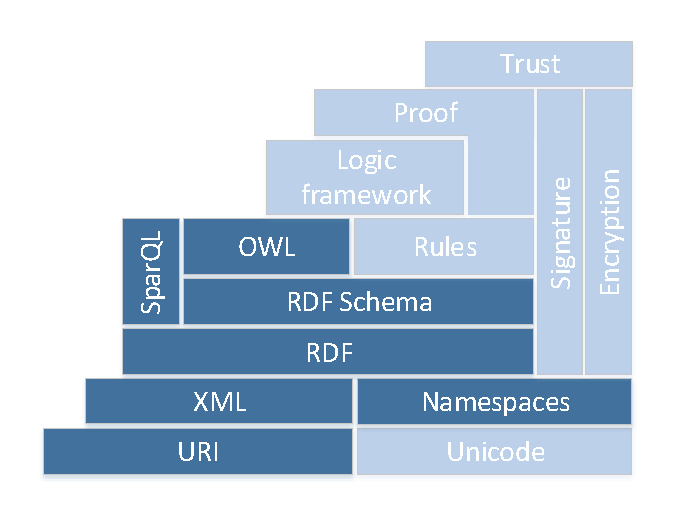
\includegraphics[width=10cm]{images/sweb-stack2.pdf}
\caption{Vuonna 2005 esitetty arkkitehtuuri. Lähde: \cite{stack}. \label{images/sweb-stack2.pdf}}
\end{figure}

Mallista on himmennetty osa-alueet, joita ei käsitellä tässä työssä. Pinomallista voidaan havaita, että semanttinen web koostuu useista eri tekniikoista. Seuraavissa alaluvuissa syvennytään pinomallissa esitettyihin tekniikoihin aloittaen pinon pohjalta. Perusteet on tärkeä ymmärtää, jotta voi löytää syitä korkeatasoisempien tekniikoiden tarpeellisuudelle.

\subsection{Resursseihin viitataan URI:eilla}
Semanttisessa webissä tietoon viitataan aina Uniform Resource Identifierin eli URI:n avulla \cite{RDF_specification}. Tämän ansiosta kaikki viittaukset tiedonkohteisiin eli resursseihin ovat yksiselitteisiä, jolloin väärinymmärrysten vaaraa ei ole. URI:eja ovat esimerkiksi URL (Uniform Resource Locator), ISBN, sähköpostiosoite ja puhelinnumero. Usein kuitenkin suositaan HTTP-protokollan mukaisia URI:eja (eli käytännössä URL:eja), jotta käyttäjä voi helposti tarkistaa mihin tunnisteella viitataan \cite{cambridge_linked}. Resurssit voivat olla mitä tahansa semanttisen webin standardeilla määritettyä tietoa, kuten esimerkiksi tekstidokumentteja tai fyysisiä laitteita \cite{RDF_specification}.

\subsection{XML-merkintäkieli}
XML (eXtensible Markup Language) on W3C:n standardoima merkintäkieli, jonka avulla voidaan tallentaa- ja siirtää tietoa. XML-merkintäkieli on suunniteltu ihmisen ja tietokoneen luettavaksi. Merkinnältään XML muistuttaa hyvin paljon HTML-merkintäkieltä (Hypertext Markup Language). XML kuitenkin eroaa HTML:stä käyttötarkoitukseltaan. XML on suunniteltu mielivaltaisen tiedon tallennuskieleksi, kun taas HTML:llä pystytään esittämään ainoastaan ennalta määriteltyjä web-sivuja \cite{IEEE_XML}. XML mahdollistaa tiedon välittämisen yksittäisessä standardoidussa muodossa. Tämän ansiosta sovellukset voivat ymmärtää toisiaan, mikäli ne tukevat XML-standardia. Alla esimerkki XML-syntaksista:
\vspace{0.3cm}
\begin{lstlisting}[style=codeblock,caption={XML-syntaksiesimerkki.},captionpos=b,label={xml-esim}]
<computer>
  <cpu>i5-4200m</cpu>
</computer>
\end{lstlisting}

 Semanttisen webin näkökulmasta XML-merkintäkieli on ongelmallinen. Edellisestä esimerkistä voidaan havaita, että prosessori on sijoitettu XML-puussa tietokone-elementin sisälle, mutta muuten merkintä on melko epämääräinen. Pelkän merkinnän pohjalta ei ole mahdollista tietää mihin tietokoneeseen viitataan, sekä prosessorin ja tietokoneen suhdetta ei voida tuntea. Ihminen tekee intuitiivisen päätelmän, että tietokone varmaankin käyttää prosessoria toimiakseen, mutta näin ei välttämättä ole. XML-merkintä ei siis sisällä riittävästi tietoa, jotta se voisi toimia semanttisen webin merkintäkielenä \cite{IEEE_XML}. XML on kuitenkin ollut lähtökohta sopivan syntaksin kehityksessä, mikä tekee siitä merkittävän merkintäkielen semanttisen webin näkökulmasta.

 \subsection{Nimiavaruudet}
 Etuliite eli prefiksi (engl. prefix) määrää käytettävän nimiavaruuden (engl. namespace). Prefiksien käyttämisestä seuraa useita hyötyjä. Dokumenteista tulee siistimpiä ja helpompia lukea, koska tekstiriveistä tulee lyhyempiä. Pitkiä URI:eja ei tarvitse toistaa jokaisen RDF-lauseen alussa, koska tarpeelliseen URI:iin viittaaminen tehdään lyhyellä prefiksillä. Prefiksien käyttö nopeuttaa dokumenttien kirjoitusprosessia, koska lyhyen etuliitteen kirjoittaminen on huomattavasti nopeampaa kuin kokonaisen URI:n. Nimiavaruudet myös sallivat samannimisten termien käytön useissa eri konteksteissa, mikä on hyvin tärkeä ominaisuus \cite{Antoniou}.

 Sama termi voi esiintyä dokumentissa useita kertoja, mutta termillä ei välttämättä aina viitata samaan asiaan. Jotta kaksi samannimistä, mutta eri asiaa tarkoittavaa termiä voidaan erottaa toisistaan, täytyy hyödyntää nimiavaruuksia. Esimerkiksi nimellä Punainen viiva voidaan viitata sekä kirjaan, että elokuvaan. Mikäli elokuvia ja kirjoja sisältävät dokumentit halutaan yhdistää, niin niissä käytetyt nimet tulisi pystyä erottamaan toisistaan, jotta tieto ei mene sekaisin. Nimien erottamiseen voidaan hyödyntää nimiavaruuksia. Elokuvat voidaan määritellä \textit{elokuva}-etuliitteen avulla ja kirjat vastaavasti \textit{kirja}-prefiksillä. Siten lopullisessa dokumentissa esiintyisi: \textit{elokuva:Punainen\_viiva} ja \textit{kirja:Punainen\_viiva}.

 Etuliitteet määritellään yleensä dokumenttien alussa, jolloin niitä voidaan käyttää määritelmien jälkeen. Prefiksin saa valita vapaasti, kunhan kyseinen etuliite ei ole jo valmiiksi käytössä. Etuliitteet täytyy siis kyetä erottamaan toisistaan, minkä vuoksi ne ovat uniikkeja. Prefiksin URI:n täytyy osoittaa olemassa olevaan resurssiin, jotta nimiavaruuden määritykset on mahdollista löytää.

\subsection{RDF-tietomalli}
%%s.18 primer
Resource Description Framework (RDF) on semanttisen webin keskeinen tietomalli. RDF on suunniteltu kuvaamaan internetissä esiintyvää tietoa niin, että metatieto ei menetä koskaan merkitystään \cite{RDF_specification}. Lisäksi RDF pyrkii sovellus riippumattomuuteen, jolloin sen avulla voidaan kuvata lähes kaikentyyppistä tietoa \cite{RDF_specification}. Tämän ansiosta RDF-tietomalli soveltuu kaikille aloille käytettäväksi, jolloin merkityksellistä metatietoa syntyy laaja-alaisesti ja paljon. Metatiedosta on hyötyä niille, jotka pystyvät tulkitsemaan sitä. Vapaasti käytettävä ja standardoitu RDF-tietomuoto on kaikkien ihmisten ja tietokoneiden hyödynnettävissä, joten RDF-metatieto edistää kaikkia \cite{metadata}. RDF-tietomuotoa hyödynnetään esimerkiksi digitaalisten valokuvien metatiedon tallennukseen \cite{XMP1} \cite{profium_metadata}.

RDF-tietomalli sisältää kuvauksia resurssien välisistä suhteista. Suhteita kutsutaan \textit{predikaateiksi} tai vaihtoehtoisesti \textit{ominaisuuksiksi} \cite{Antoniou}. Predikaatit täytyy määritellä tietokoneelle erikseen, koska tietokone ei kykene luomaan niitä itsestään. Predikaatilla voidaan liittää kaksi resurssia yhteen ilmaisten resurssien välisestä suhteesta. Esimerkiksi predikaatilla \textit{omistaa} voidaan kuvata resurssien liitos: pankinjohtaja omistaa talon. (Huomaa, että oikeaoppisesti pankinjohtajaan ja taloon pitäisi viitata URI:en avulla). Edellinen kuvaus siis määrittää tietyn pankinjohtajan ja tietyn talon välille omistusliitoksen.

\subsubsection{RDF-toteamukset}
\textit{Toteamukset} (engl. statements) ovat RDF-tietomallin pääasiallinen tapa esittää tietoa. Toteamukset voidaan kuvata resurssien, predikaattien ja määriteltyjen arvojen avulla \cite{Antoniou}. Esimerkiksi \textit{auto ajaa 100 km/h} on toteamus, joka voidaan esittää RDF-tietomallilla. Esitetyn arvon ei tarvitse olla lukuarvo, vaan se voi olla myös toinen resurssi, kuten edellisen kappaleen omistusliitos esimerkissä on tehty \cite{Antoniou}\cite{IEEE_XML}. Toteamukset sisältävät paljon tietoa ja esitysmuoto on hyvin joustava, minkä vuoksi RDF-tietomallilla voidaan kuvata monenlaista tietoa.

Toteamus rakentuu \textit{subjektista}, \textit{predikaatista} ja \textit{objektista} \cite{lassila_dissertion}. Rakenteensa vuoksi toteamuksia voidaan myös nimittää \textit{kolmikoiksi} (engl. triple). Kolmikkoja voidaan esittää graafimuodossa kuvan \ref{images/RDF-triplet1} tapaan. Kaaviot saattavat auttaa hahmottamisessa, minkä vuoksi niitä käytetään havainnollistamisen tukena. On kuitenkin hyvä tiedostaa, että graafien esittämiseen ei ole määritelty standardia, joten tässä työssä käytetyt graafit ovat vain yksi monista mahdollisista esitysmuodoista. Lisäksi on hyvä ymmärtää, että resursseihin täytyy aina viitata URI:en avulla, mutta selkeyden vuoksi graafeissa saattaa esiintyä ainoastaan yksittäisiä sanoja.

%% Graafi
\begin{figure}[htb]
\centering
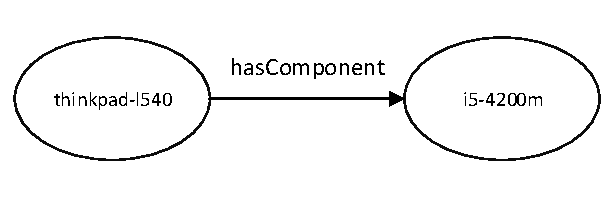
\includegraphics[height=3cm]{images/RDF-triplet.pdf}
\caption{Esimerkki kolmikosta. \label{images/RDF-triplet1}}
\end{figure}

Kaaviossa esitetään toteamus: \textit{computer hasComponent cpu}. \textit{Computer} on toteamuksen subjekti ja \textit{cpu} on objekti. Predikaatin asemassa on \textit{hasComponent}, jonka avulla ilmaistaan, että tietokone sisältää komponentin cpu. Yhdessä edelliset toteamuksenjäsenet muodostavat kolmikon.



\subsubsection{RDF/XML-syntaksi}
RDF/XML on syntaksi, jonka avulla tietokoneelle voidaan esittää RDF-tietomallin mukaista tietoa. RDF/XML-syntaksi määrää tiedon esitysmuodon, jolloin tietokone ymmärtää ihmisen esittämän tiedon halutulla tavalla. Syntaksi pohjautuu XML:ään \cite{RDF_XML}. Alla on esitetty edellisen graafin (Kuva \ref{images/RDF-triplet1}) toteamus RDF/XML-merkintäkielellä:

%% XML/RDF example
%% hasProduct instead of product?
\vskip 0.75cm
\begin{lstlisting}[style=codeblock,caption={RDF/XML syntaksiesimerkki.},captionpos=b,label={rdf_esim}]
<?xml version="1.0"?>
<rdf:RDF
xmlns:rdf="http://www.w3.org/1999/02/22-rdf-syntax-ns#"
xmlns:rel="http://www.cmspecs.com/relationships">

<rdf:Description rdf:about="http://www.cmspecs.com/computers/thinkpad-l540">
    <rel:hasComponent rdf:resource="http://www.cmspecs.com/processors/i5-4200m"/>
</rdf:Description>
</rdf:RDF>
\end{lstlisting}
% \vspace{-1pc}
% See code~\ref{lst:label}
\vskip 0.75cm

\begin{figure}[htb]
\centering
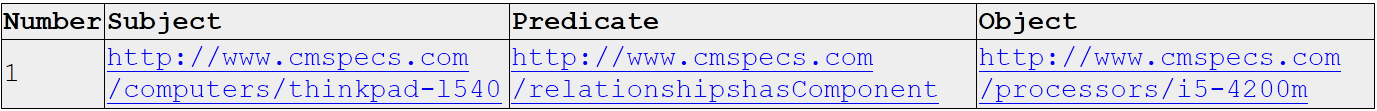
\includegraphics[width=15cm]{images/RDF-valid.PNG}
\caption{Suhteet taulukoituna. Lähde: \cite{W3C_RDF_validator}. \label{images/RDF-valid}}
\end{figure}

Yllä oleva taulukko (Kuva \ref{images/RDF-valid}) on generoitu automaattisesti RDF/XML-merkinnän pohjalta käyttämällä W3C:n validointipalvelua. Voimme havaita, että ulkopuolinen palvelu on ymmärtänyt esimerkin rakenteen täysin oikein. Validaattori on löytänyt subjektiksi tietokoneen (\textit{thinkpad-l540}), objektiksi prosessorin (\textit{i5-4200m}) ja predikaatiksi \textit{hasComponent}-suhteen. Esimerkin RDF/XML-syntaksi on siis mahdollistanut tietokoneen ymmärtää ihmisen esittämää tietoa halutulla tavalla. Nyt tietokoneet kykenevät siis havaitsemaan \textit{thinkpad-l540}:n ja \textit{i5-4200m}:n välillä vallitsevan yhteyden.


\subsubsection{Turtle-syntaksi}
Nykyisin RDF:ää kirjoitettaessa suositaan paljon muitakin syntakseja kuin pelkkää RDF/XML:ää. Esimerkiksi Turtle (Terse RDF Triple Language) on hyvin suosittu syntaksi sen helpon luettavuuden ja kirjoitettavuuden vuoksi \cite{cambridge2}. Turtlessa toteamukset päättyvät pisteeseen. Alla on esitetty edellinen tietokone--prosessori esimerkki Turtle-syntaksilla:

%%Turle example
\vskip 0.75cm
\begin{lstlisting}[style=codeblock,caption={Turtle syntaksiesimerkki.},captionpos=b,label={turtle_esim}]
@prefix rdf: <http://www.w3.org/1999/02/22-rdf-syntax-ns#> .
@prefix rel: <http://www.computerspecs.com/semantics/relationships> .
@prefix computer: <http://www.computerspecs.com/semantics/computers> .
@prefix cpu: <http://www.computerspecs.com/semantics/processors> .

computer:thinkpad-l540 rel:hasComponent cpu:i5-4200m .

\end{lstlisting}
\vskip 0.75cm

\begin{figure}[htb]
\centering
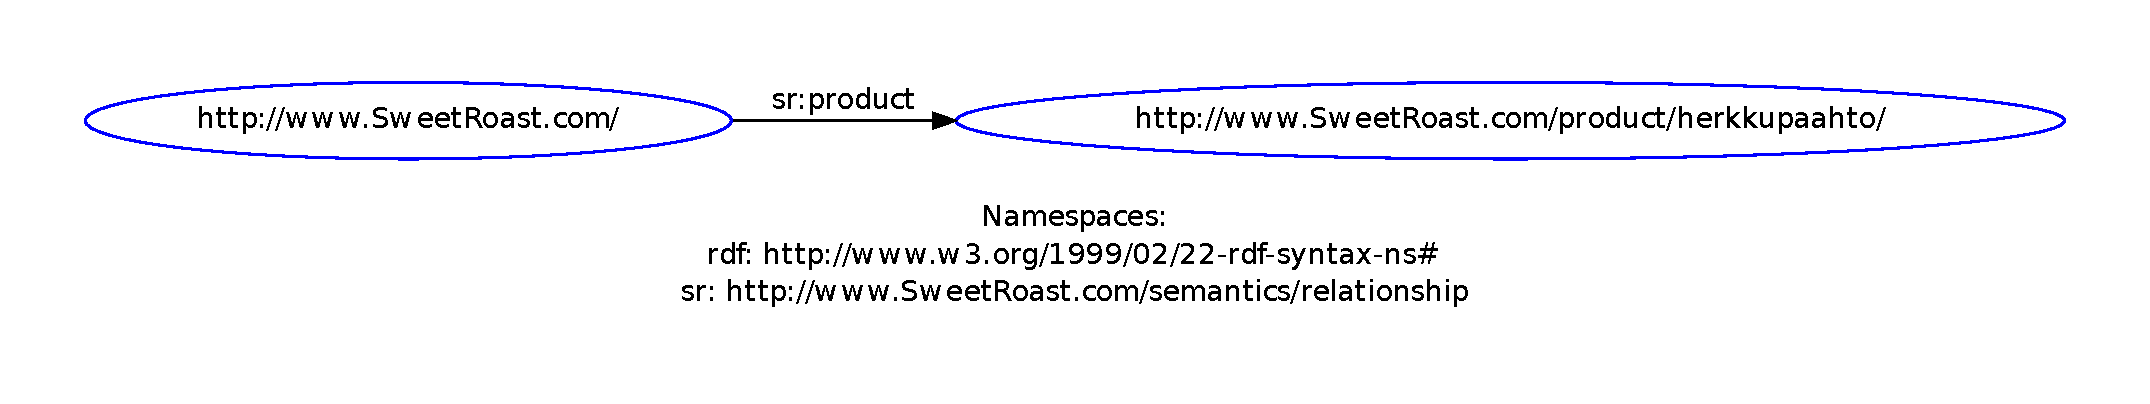
\includegraphics[width=15cm]{images/RDF-triplet2.pdf}
\vspace{-3pc}
\caption{Turtle-syntaksista automaattisesti generoitu graafi. Lähde: \cite{SeCo_RDF_validator} \label{images/RDF-triplet2}}
\end{figure}

Vaikka edelliset syntaksiin liittyvät esimerkit ovat minimaalisia, voidaan niistä silti havaita Turtlen selkeys ja tiiveys verrattuna RDF/XML-merkintään. Turtlella RDF-toteamus voidaan kirjoittaa yhdelle riville. Subjektista, objektista ja predikaatista koostuva kolmikko päätetään aina pisteeseen tai puolipisteeseen.

\subsection{Semanttinen tieto}
Filosofia määrittelee termin {\textit{semantiikka} yleiseksi teoriaksi sanojen, ilmaisujen ja lauseiden merkityksestä \cite{semantics_phi}. Tietotekniikan tutkimusala on omaksunut termin käyttöönsä. Semantiikka ei määrittele tiedon esitysmuotoa, joten suomenkielisten lauseiden sijaan voidaan myös tutkia RDF-tietomallin mukaisia toteamuksia. Semantiikan näkökulmasta on mielenkiintoista, kuinka tietoa voidaan esittää niin, että tiedon merkitys ymmärretään yksiselitteisesti. Semanttinen web pyrkii erityisesti esittämään ihmiseltä peräisin olevaa tietoa niin, että tietokone ymmärtää tiedon samalla tavalla kuin ihminen \cite{Berners_visio}.

Luonnollinen kieli (ihmiskieli) sisältää paljon tietoa, jota on vaikea esittää tietokoneelle \cite{semantics}. Esimerkiksi lauseesta ``\textit{En voi ajaa tuota autoa yhdellä jalalla}'' ihminen voi tehdä useita päätelmiä. Kokonaisesta lauseesta voidaan esimerkiksi päätellä:
\begin{itemize}
  \item  Lause kertoo jostain tietystä autosta, joten ehkä lauseenkertoja osoittaa autoa.
  \item  Lauseesta käy ilmi puhujan kyvyttömyys tietyn auton ajamiseen. Ehkä auto on vääränmallinen (esim. auto on manuaalivaihteinen automaatin sijaan).
  \item  Lauseessa esiintyvä jalka on mitä luultavimmin puhujan.
  \item  Lauseessa puhutaan yhdestä jalasta, joten ehkä puhujan toiselle jalalle on käynyt jotain.
\end{itemize}
Lauseiden sanajärjestyksellä on myös oma merkityksensä. Esimerkiksi lauseet \textit{lapset söivät keksit} ja \textit{keksit söivät lapset} eivät tarkoita samaa, vaikka ne koostuvatkin täysin samoista sanoista \cite{semantics}. Kokonaiset lauseet ovat siten informatiivisempia kuin sanoista erikseen pääteltävissä oleva informaatio. Tästä syystä RDF-tietomuodon lauserakenne on tehokas kuvaamaan tietoa. Käytännössä tietokoneelle esitetyt toteamukset eivät voi kuitenkaan olla yhtä tietorikkaita kuin edellinen esimerkkilause, koska tietoa täytyy pystyä käsittelemään logiikan avulla ja RDF-toteamukset koostuvat ainoastaan subjektista, predikaatista ja objektista.

Semanttisella tiedolla viitataan tietoon, josta selviää itse tiedon lisäksi myös sen merkitys. Jotta voi ymmärtää merkityksiä, täytyy kyetä tunnistamaan tiedon välisiä suhteita. Semanttisen webin yhteydessä semanttisella tiedolla tarkoitetaan tietoa, jonka esittämiseen hyödynnetään Semanttisen webin tekniikoita. Tekniikat mahdollistavat tiedon suhteiden ja siten merkityksien kuvaamisen tietokoneelle. Tiedon suhteita voidaan esittää esimerkiksi luokkamäärittelyjen ja luokkahierarkioiden avulla. Semanttisen webin tekniikoilla esitetty tieto on myös formaalia, koska tietokone kykenee lukemaan ja prosessoimaan tietoa loogisten kuvausten ansiosta. Semantiikan esittäminen siis mahdollistaa päättelyn tietokoneelle.


\subsection{RDF Schema}
%%Usein tietoa halutaan kuvata tarkasti, jolloin RDF:n tukena tulee käyttää RDF Schemaa.
RDF Schema (Resource Description Framework Schema) mahdollistaa tietojoukkojen ja toisiinsa liittyvien resurssien kuvailun. RDFS tarjoaa RDF:n jatkeena lisämahdollisuuksia tiedon kuvailuun. Esimerkiksi luokkamäärittelyt ovat yksi erittäin tärkeä RDFS:n työkalu, joka mahdollistaa tiedon kuvailun yleisellä tasolla \cite{W3C_RDFS2}. RDF Scheman avulla voidaan kuvata esimerkiksi talojen yleisiä ominaisuuksia määrittelemällä \textit{talo}-luokan, kun taas RDF:llä pystytään kuvaamaan ainoastaan yksittäisten tunnettujen talojen ominaisuuksia \cite{Antoniou}. RDF Schema on kirjoitettu RDF-tietomallin avulla, minkä vuoksi RDFS:ää hyödyntävät sovellukset ovat myös valideja RDF-sovelluksia \cite{RDF_specification_old}.

Luokkien määrittäminen auttaa järjellisen tiedon esittämisessä. Luokkien avulla voidaan luoda rajoitteita liittyen RDF-väitteisiin, mikä estää mielettömien väitteiden esittämisen. Voimme esimerkiksi määritellä \textit{kirjoittaja}-ominaisuuden, joka kuuluu ainoastaan \textit{kirja}-luokalle. Tämän jälkeen voidaan todeta, että kirjan \textit{Sinuhe} kirjoittaja on henkilöluokkaan kuuluva \textit{Mika Waltarin}. Määrittely kuitenkin estää esittämästä järjettömiä toteamuksia: \textit{Helsingin kirjoittaja on Mika Waltarin}. \textit{Helsinki} on kaupunki ja kaupungilla ei ole kirjoittajaa, joten sen kirjoittaja ei voi olla \textit{Mika Waltarin}. Semanttinen tieto siis mahdollistaa päättelyiden tekemisen ja ristiriitaisuuksien havaitsemisen \cite{Antoniou}.

%% \textcolor{red} {RDF Schemassa luokan ominaisuudet kuvataan resurssikohtaisesti}
RDFS:n luokat muistuttavat luokkapainotteisten olio-ohjelmointikielten luokkia. Selvänä erona on kuitenkin tapa, jolla luokan ominaisuudet määritetään. Tavallinen ohjelmointikieli voi määrittää esimerkiksi luokan \textit{auto} koostuvan \textit{renkaista}, \textit{ovista} ja \textit{moottorista}. Kun luokasta luodaan autoinstanssi, niin sillä ilmenee aina edelliset ominaisuudet. RDF Schemassa luokkien ominaisuudet kuvataan globaalissa nimiavaruudessa ja ominaisuudet sidotaan sopiviin resursseihin \textit{domain} ja \textit{range} mekanismien avulla. Siten käyttäjät voivat jatkaa toistensa tekemiä luokkia, vaikka heillä ei olisi mahdollisuutta muokata alkuperäistä luokkamääritelmää \cite{Antoniou} \cite{W3C_RDFS2}.

Tärkeitä RDFS:n ominaisuuksia ovat muun muassa \textit{domain}, \textit{range} ja \textit{subClassOf}, joilla on vahva yhteys luokkiin. \textit{Domainin} avulla voidaan määrittää tietyn ominaisuuden kuuluvan tietylle luokalle. Voidaan esimerkiksi määrittää \textit{auto}-luokka ja predikaatti \textit{hasMotor}. \textit{Domainin} avulla voidaan kertoa, että \textit{hasMotor}-predikaatti kuuluu \textit{auto}-luokalle, joten predikaattia on mieletöntä käyttää kuvailemaan esimerkiksi auton \textit{rengasta}. \textit{Rangen} avulla määritetään mihin predikaatilla voidaan viitata. Edellisen esimerkin tapauksessa olisi järkevää määrittää \textit{hasMotor}-predikaatin \textit{rangeksi} \textit{moottori}-luokka. Siten auton \textit{moottori} voi olla ainoastaan \textit{moottori}-luokan ilmentymä (engl. instance). RDFS:n \textit{subClassOf} ominaisuuden avulla voidaan esitellä alaluokkia, mikä mahdollistaa luokkahierarkioiden kuvaamisen. \textit{Auto}-luokan alaluokka voisi olla esimerkiksi \textit{sedan}
\cite{W3C_RDFS2}.

Seuraavassa esimerkissä (koodikatkelma \ref{rdfs_esim} ja graafi \ref{images/laptop}) käytetään edellisessä kappaleessa esiteltyjä RDFS-ominaisuuksia. Esimerkissä määritetään luokat: \textit{akku}, \textit{tietokone} ja \textit{kannettava tietokone} ja ominaisuudet: \textit{hasBattery}, \textit{hasVoltage} ja \textit{hasPower}. Tämän jälkeen luodaan \textit{Akku} ja \textit{kannettava tietokone} ilmentymät, joita kuvataan edellisillä ominaisuuksilla. Alla oleva graafi selventää tilannetta. Koodikatkelma on kirjoitettu Turtle-syntaksilla. Esimerkissä hyödynnetään Turtlen tarjoamaa mahdollisuutta lyhentää toteamuksia määrittelemällä niiden subjekti ainoastaan kerran. Puolipisteen jälkeiset toteamukset viittaavat edelleen samaan subjektiin, kun taas pisteen jälkeen täytyy määritellä aina uusi subjekti.

\begin{figure}[htb]
\centering
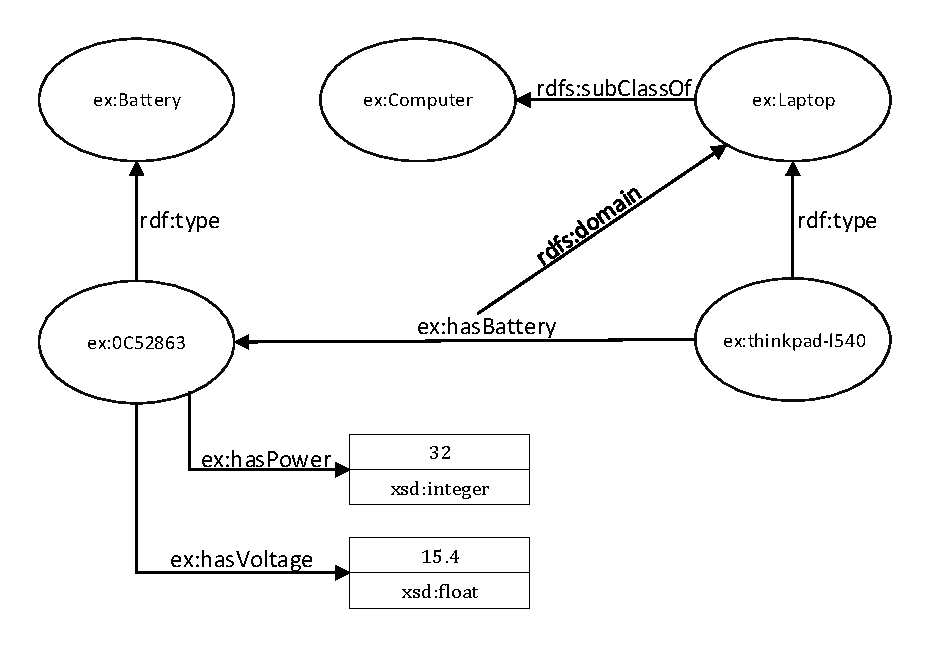
\includegraphics[width=15cm]{images/laptop.pdf}
\vspace{-3pc}
\caption{RDFS esimerkin graafi}
\label{images/laptop}
\end{figure}
%% RDFS
\vskip 0.75cm
\begin{lstlisting}[style=codeblock,caption={RDFS esimerkki.},captionpos=b,label={rdfs_esim}]
@prefix ex: <http://www.computerspecs.com/semantics/example> .
@prefix rdf: <http://www.w3.org/1999/02/22-rdf-syntax-ns#> .
@prefix rdfs: <http://www.w3.org/2000/01/rdf-schema#> .
@prefix xsd: <http://www.w3.org/2001/XMLSchema#> .

# Class definitions
ex:Battery  rdf:type rdfs:Class .
ex:Computer rdf:type rdfs:Class .
ex:Laptop   rdf:type rdfs:Class ;
    rdfs:subClassOf ex:Computer .

# Data properties
ex:hasBattery a rdf:Property ;
    rdfs:domain ex:Laptop ;
    rdfs:range  ex:Battery .

# Instances
ex:0c52863 a ex:Battery ;
    ex:hasPower "32"^^xsd:integer ;
    ex:hasVoltage "15.4"^^xsd:float .

ex:thinkpad-l540 a ex:Laptop ;
    ex:hasBattery ex:0C52863 .


\end{lstlisting}

\subsection{OWL}
% KIRJOITA: OWL on logiikkapohjainen kieli, mikä sallii tietokoneiden käsitellä ilmaisuja.
% https://www.w3.org/OWL/

OWL (Web Ontology Language) on semanttisen webin yhteydessä käytetty tietämyksenesittämiskieli. Tietämyksenesittämiskielille tärkeitä ominaisuuksia ovat selkeästi määritelty syntaksi, formaali semantiikka, riittävä ilmaisuvoima ja päättelytuki \cite{Antoniou}. Käyttötarkoitukseltaan OWL on rinnastettavissa RDF Schemaan, mutta ilmaisuvoimaltaan OWL on huomattavasti tehokkaampi kuin RDFS. RDF Schema tarjoaa ainoastaan vähimmäisedellytykset semanttisen tiedon kuvaamiseen \cite{revisited}. OWL:sta on tarjolla kolme erilaajuista versiota: OWL Full, OWL DL ja OWL Lite. OWL Full on kaikista laajin versio ja monet sovellukset eivät tue sitä kokolaajuudessaan \cite{OWL_specification}.

Formaalilla semantiikalla tarkoitetaan kykyä ilmaista esitetyn tiedon merkitys tarkasti ja yksiselitteisesti \cite{Antoniou}. Tämä mahdollistaa päättelyn esitetyn tiedon pohjalta. Esimerkiksi \textit{joutsen}-alaluokkaan kuuluva \textit{laulujoutsen} kuuluu selvästi myös \textit{lintuluokkaan}, ja siten omaa linnulle tyypillisiä ominaisuuksia. Päätelmä voi olla tarpeellinen esimerkiksi sovelluksessa, joka kuvailee eläintyypin tavanomaisia ominaisuuksia, kun tarkastellaan eläinlajia. OWL tarjoaa monia erilaisia keinoja pääteltävän tiedon määrittelyyn, mikä tekee siitä ilmaisuvoimaisen.

Owl määrittelee muun muassa funktionaalisen, transitiivisen ja symmetrisen luokkaominaisuuden. Edelliset ominaisuudet eivät ole ainoita OWL:n ominaisuuksia, mutta niiden tarkoitus on antaa lukijalle riittävä mielikuva OWL:n tarjoamista mahdollisuuksista määritellä tietoa. Funktionaalisella ominaisuudella tarkoitetaan instanssien välistä suhdetta, jossa instanssia kohden voi ilmetä ainoastaan yksi uniikki arvo. Esimerkiksi auton ja rekisterinumeron välistä suhdetta voidaan kuvata funktionaalisella ominaisuudella. Transitiivisella ominaisuudella voidaan kuvata pääteltäviä osakokonaisuussuhteita. Esimerkiksi \textit{pöydänjalan} ollessa \textit{pöydän} osa ja \textit{ruuvin} ollessa \textit{pöydänjalan} osa, voidaan päätellä, että \textit{ruuvi} on myös \textit{pöydän} osa. Symmetrisellä ominaisuudella viitataan ystävyyssuhdetta vastaavaan ilmentymään. Yleensä kaverukset kokevat toisensa ystävikseen, joten suhde on molemminpuolinen eli symmetrinen \cite{OWL_specification}.

Seuraavassa esimerkissä (koodikatkelma \ref{owl_esim}) on esitetty RDF Schema luvun kannettava tietokone -esimerkki täydennettynä OWL:lla. Esimerkistä voidaan huomata, että se näyttää edelleen hyvin samalta kuin aiemmin. OWL-määritelmät ovat lisätietoa. Esimerkin Turtle-merkintä on generoitu Protégé-nimisellä ohjelmistolla, jonka avulla voidaan tuottaa ontologioita tehokkaasti \cite{Protege}.

\vskip 0.75cm
\begin{lstlisting}[style=codeblock,caption={OWL esimerkki.},captionpos=b,label={owl_esim}]
@prefix : <http://www.Computer-Specs.com/ontologies/example#> .
@prefix owl: <http://www.w3.org/2002/07/owl#> .
@prefix xml: <http://www.w3.org/XML/1998/namespace> .
@prefix xsd: <http://www.w3.org/2001/XMLSchema#> .
@prefix rdf: <http://www.w3.org/1999/02/22-rdf-syntax-ns#> .
@prefix rdfs: <http://www.w3.org/2000/01/rdf-schema#> .
@base <http://www.Computer-Specs.com/ontologies/example> .

<http://www.Computer-Specs.com/ontologies/example> rdf:type owl:Ontology .

# Object Properties
:hasBattery rdf:type owl:ObjectProperty ;
            rdfs:domain :Laptop ;
            rdfs:range :Battery .

# Data properties
:hasPower rdf:type owl:DatatypeProperty ;
          rdfs:domain :Battery .

:hasVoltage rdf:type owl:DatatypeProperty ;
            rdfs:subPropertyOf owl:topDataProperty ;
            rdfs:domain :Battery .

# Classes
:Battery  rdf:type owl:Class .
:Computer rdf:type owl:Class .
:Laptop   rdf:type owl:Class ;
          rdfs:subClassOf :Computer .

# Individuals
:C52863 rdf:type owl:NamedIndividual ;
        :hasPower "57"^^xsd:int ;
        :hasVoltage "10.8"^^xsd:float .

:thinkpad-l540 rdf:type owl:NamedIndividual ,
                           :Laptop ;
               :hasBattery :0C52863 .

\end{lstlisting}
\vskip 0.75cm

\subsection{Ontologiat ja sanastot}

% An ontology is a formal, explicit specification of a shared conceptualisation \cite{ontology_def}.
Vuonna 1998 Studer et al. määritteli ontologian seuraavasti: ``Ontologia on formaali, eksplisiittinen määritelmä yhteisestä käsitteellistämisestä.'' \cite{ontology_def}. Yhteisellä käsitteellistämisellä hän viittaa kaikkien saatavilla olevaan malliin jostakin maailman ilmiöstä, minkä merkitykselliset konseptit kyetään tunnistamaan ja ilmaisemaan käsitteiden avulla \cite{ontology_def}. Edellinen määritelmä tiivistää ontologia-käsitteen tarkoituksen tehokkaasti, mutta määritelmää voi olla vaikeaselkoinen, mikäli ontologia-käsitettä ei tunne entuudestaan. Ontologiat voidaan ymmärtää kokoelmina toteamuksia, jotka määräävät konseptien välisiä suhteita ja määrittelevät loogisia sääntöjä, joiden avulla tiedosta voidaan tehdä päätelmiä \cite{Berners_visio}. Termillä \textit{sanasto} (engl. vocabulary) voidaan viitata samaan asiaan kuin ontologialla \cite{vocabulary}.

Ontologiat ovat usein rakenteeltaan monimutkaisia, formaaleja ja laajoja. Jos rakenne on kuitenkin melko yksinkertainen, niin ontologian sijaan käytetään usein termiä sanasto. Toisinaan sanaston ja ontologian erottaminen voi olla hyvin haastavaa, minkä vuoksi termejä voidaankin käyttää myös toistensa synonyymeinä \cite{vocabulary}. Sekä ontologioiden että sanastojen toimivuuden kannalta on tärkeää, että määrittelyt tehdään tietokoneluettavassa muodossa ja yksiselitteisesti. Yksiselitteisen eli eksplisiittisen määrittelyn seurauksena tieto täytyy kuvata sovelluskohtaisesti, jotta jokaisella termillä on vain ja ainoastaan yksi merkitys \cite{RDF_specification}. Luonnollisessa kielessä yhdellä sanalla voi olla monia merkityksiä, mutta ylimääräisistä merkityksistä päästään eroon, kun termi määritellään sovelluskohtaisesti. Tietokoneluettava ja eksplisiittinen konseptien määrittely tehostaa ihmisen ja tietokoneen välistä kommunikointia \cite{ontology_learning}. Lisäksi tietokoneen ymmärtämä termistö ja semantiikka mahdollistavat päättelyn tiedon pohjalta.

Ontologioita ja sanastoja voidaan kirjoittaa OWL:n ja RDF Scheman avulla. Ontologioilla voidaan määritellä sovellukselle ominaisia tiedon rakenteita ja rajoitteita. \cite{vocabulary}. Esimerkiksi rakennussovellusta varten voitaisiin määritellä \textit{yhteensopiva}-predikaatti, sekä erilaisia \textit{mutteri} ja \textit{pultti} resursseja. Tämän jälkeen voitaisiin määritellä, että saman kierteen omaavat \textit{pultit} ja \textit{mutterit} ovat yhteensopivia, minkä seurauksena sovelluksen käyttöliittymä voisi tarjota käyttäjälle ainoastaan yhteensopivia rakennustarvikevaihtoehtoja. Hyvin määriteltyjä sanastoja ja ontologioita voidaan uudelleen käyttää ja jakaa muiden kesken. Esimerkiksi Dublin Core ja Friend of a Friend (FOAF) ovat todella tunnettuja ja maailmanlaajuisesti RDF:n yhteydessä käytettyjä ontologioita \cite{data_namespace}.

Sanastoja ja ontologioita hyödynnetään myös tiedon integroinnissa ja organisoinnissa \cite{vocabulary}. Esimerkiksi tuotteen maahantuojan tuotetietojen ja kauppiaan myynti tietojen yhdistäminen voi olla hyödyllistä. Kauppiaan ei tarvitse kuvailla myymien tuotteidensa ominaisuuksia, koska hän voi hyödyntää maahantuojan valmiita kuvauksia. Kauppias ja myyjä eivät kuitenkaan todennäköisesti kuvaile tuotteita täysin samalla RDF-termistöllä. Siksi tarvitaan sanasto, jonka avulla voidaan esittää tarpeellinen termien yhdistämiseen vaadittava lisätieto. Ilman sanastoa tietokone ei kykenisi yhdistämään maahantuojan tuotekuvausta ja myyjän vastaavaa tuotetta toisiinsa \cite{vocabulary}.


\subsection{RDF-muotoisen tiedon tallentaminen}


\subsubsection{Triplestore}
RDF-tietomuodossa olevaa tietoa voidaan tallentaa muistiin. Yksinkertaisimmillaan voidaan tallentaa suoraan RDF/XML-, Turtle- tai vastaavia tiedostoja, mutta tämä ei ole kovin tehokasta. Yksittäisen tarpeellisen asian etsiminen on hidasta, kun tiedostokoot ovat suuria. Tästä syystä on kehitetty tehokkaampiakin tallennustapoja, jotka hyödyntävät tietokantoja. Triplestore on tietokantatyyppi, joka on suunniteltu erityisesti RDF-graafien tallentamiseen. RDF-tieto on todella linkittynyttä, minkä vuoksi graafi-tietokannat soveltuvan sen tallentamiseen paremmin kuin perinteiset relaatiotietokannat. Relaatiotietokannoissa useiden linkittyneiden alkioiden välille on huomattavasti vaikeampaa luoda suhderakenteita ja kyselyiden tekeminen on myös haastavaa \cite{triplestore2}. Triplestore -tietokanta tallentaa RDF-lauseet suoraan kolmikkoina, joten sovelluskohtaisia relaatiotauluja ei tarvitse luoda \cite{triplestore}. Triplestoren yksinkertainen rakenne ja tarkka standardointi sallivat tietokantojen liittämisen toisiinsa vaivattomasti. Tämän ansiosta tietokantoja linkittämällä voidaan luoda suuria tietoverkkoja.


\begin{figure}[htb]
\centering
\includegraphics[width=15cm]{images/linked_data.png}
\caption{Graafi vapaasti hyödynnettävistä linkittyneistä tietokannoista vuonna 2017. (LOD cloud diagram). Lähde: \cite{LOD_cloud} \label{images/linked_data}}
\end{figure}
\clearpage

\subsubsection{SPARQL Quarey Language}
%% päätepiste???
SPARQL-kyselykielen (SPARQL Query Language) avulla voidaan hakea RDF-muotoista tietoa triplestore-tietokannoista. Kyselykieli vastaa relaatiotietokantojen SQL-kyselykieltä. Jokaisella triplestorella on SPARQL-päätepiste (engl. endpoint), johon SPARQL-kyselyt voidaan lähettää HTTP (Hypertext Transfer Protocol) protokollan avulla. Päätepisteen luominen internettiin on helppoa, joten avoimia päätepisteitä on paljon tarjolla. Esimerkiksi DBpedia tarjoaa avoimen päätepisteen (http://dbpedia.org/sparql), josta voi hakea tietoa RDF-tietomuotoisesta Wikipediasta \cite{Antoniou}.

RDF:ssa toteamukset koostuvat subjektista, predikaatista ja objektista. SPARQL-kyselylauseessa, jokin edellisistä RDF-toteamuksen osista voidaan korvata muuttujalla, mitä merkitään kysymysmerkillä muuttujanimen alussa \cite{Antoniou}. SPARQL etsii kyselylausetta vastaavat toteamukset ja palauttaa niistä muuttujan paikalle sopivat arvot. Kyselylause voi olla esimerkiksi seuraavanlainen:

\begin{lstlisting}[style=codeblock]
PREFIX ex: <http://www.Computer-Specs.com/ontologies/example#> .

SELECT ?battery
WHERE {
  ex:thinkpad-l540 ex:hasBattery ?battery.
}
\end{lstlisting}

Edellinen SPARQL-kysely palauttaisi käyttäjälle tunnisteen \textit{0C52863}, koska aiemmissa esimerkeissä \textit{thinkpad-l540}:n akuksi on määritelty \textit{0C52863}. Kyselyn tulos voi koostua myös useammasta kuin yhdestä arvosta, mikäli useampi toteamus toteuttaa kyselyn. SPARQL hakee tietoa prefiksien avulla määrätyistä resursseista.

SPARQL tarjoaa monia keinoja hakujen tekemiseen. Kyselyssä voi esiintyä useita muuttujia.
Haut voivat koostua yhdisteestä (engl. union) ja negaatioista. Lukuarvoista koostuva tulos voidaan summata yhteen sum-funktion avulla. Tulokset voidaan myös järjestellä haluttuun järjestykseen ORDER BY- lauseen avulla. Haku voi olla SELECT-kyselyn sijaan myös ASK-tyyppinen, joka testaa, mikäli haulla on olemassa olevia ratkaisuja ja palauttaa tuloksen mukaisen boolean-arvon \cite{sparql_query}. Erilaisia mahdollisuuksia kyselylauseiden muodostamiseen on monia. SPARQL tarjoaa useita erilaisia syntakseja kyselytuloksen esittämiseen. Kyselyn tulos voidaan esimerkiksi esittää Turtle- tai RDF/XML- syntaksin mukaisessa muodossa. \cite{W3C_turtle}.


\clearpage
%%===============================================================================

\subsection{Yhdistetty tieto}

\textit{Yhdistetty tieto} (engl. Linked data) sallii yhteisiin tietoresursseihin viittaamisen. Tietoa ei tarvitse monistaa, vaan eri tietolähteet voivat käyttää samoja tietoresursseja hyödykseen \cite{linked_data_finlad}. Tämän ansiosta tiedon tallennukseen tarvitaan vähemmän muistitilaa ja tiedon muuttaminen on nopeampaa, koska muutos täytyy tehdä ainoastaan yhteen paikkaan. Lisäksi tiedon katsotaan rikastuvan, kun siihen liitetään muuta merkityksellistä tietoa \cite{linked_data_finlad}. Saumaton ja tehokas yhdistetyn tiedon hyödyntäminen vaatii, että sovelluksen suunnittelussa noudatetaan seuraavia sääntöjä \cite{cambridge_linked}:
\begin{enumerate}
\item Resurssien nimeämiseen täytyy käyttää URI:eja.
\item URI:en tulee tukea HTTP-protokollaa, jotta ihmiset voivat selvittää URI:en merkityksen.
\item Kun käyttäjä tutkii URI:a, niin hänelle pitää tarjota merkityksellistä tietoa standardiformaatissa (esimerkiksi RDF).
\item Käyttäjälle täytyy tarjota linkkejä muihin resursseihin, jotta hän voi löytää uusia mielenkiintoisia resursseja.
\end{enumerate}
\vspace{0.5cm}

Graafimaiset tietokannat ovat merkittävässä asemassa yhdistetyn tiedon kannalta. Tavallisten relaatiotietokantojen rakenne riippuu pitkälti sovelluksesta. Koska tietokannat ovat erilaisia eri sovellusten välillä, niin tiedon hakeminen on haastavaa, mikäli tietokantaa ei tunne entuudestaan. Tästä syystä graafimaiset tietokannat soveltuvat yhdistetyn tiedon käyttöön paremmin, koska niiden rakenne ei vaihtele sovellusten kesken. Kun viittaukset resursseihin tehdään URI:en avulla, niin tietokannan käyttäjä myös tietää tarkalleen mihin resurssit viittaavat \cite{cambridge_linked}.

\clearpage
%%===============================================================================
\section{Käytännön sovelluksia}

Semanttista tietoa voidaan käyttää monella tavalla hyödyksi. Tässä kappaleessa esitellään eräitä hyödyntämismahdollisuuksia esimerkkien avulla. Esimerkit on laadittu käytössä olevista ja toimivista ratkaisuista. Jokaisessa esimerkissä yritetään painottaa eri semanttisen webin osa-aluetta. Ensimmäisessä esimerkissä käsitellään RDF-tietomuotoa, toisessa semantiikkaa ja kolmannessa ontologioita, jotka liittyvät vahvasti semantiikkaan.


\subsection{XMP-metadataformaatti}
XMP (Extensible Metadata Platform) on Adoben kehittämä metadataformaatti, jota käytetään muun muassa kuvien metadatan tallennukseen. XMP on ISO:n (International Organization for Standardization) hyväksymä standardi (ISO 16684-1:2012) \cite{XMP_standard}. XMP-merkintätekniikka pohjautuu RDF-tietomallin osajoukkoon ja se hyödyntää toteutuksessaan Dublin Core sanastoa \cite{XMP2}. Merkintäteknikan avulla tallennetaan hyödyllistä metatietoa itse tiedostoihin, jolloin tietoa kuvaileva tieto on aina saatavilla tiedostojen yhteydessä \cite{XMP1}.

XMP-metadataformaatista on useita hyötyjä. Sen avulla tiedostot säilyttävät niiden kontekstin, kun tiedostoja siirrellään ohjelmistolta, laitteelta tai tietokannasta toiseen. Yhteinen metadataformaatti mahdollistaa tiedostojen tehokkaan etsimisen eri tiedostotyyppien ja tietokantojen välillä. XMP-metadatan avulla voidaan merkitä yhteyksiä eri tiedostojen välille, mikä auttaa tiedostojen järjestelyssä. Avoimen standardin ansiosta XMP:n hyödyt ovat kaikkien saatavilla \cite{XMP_overall}. Konkreettinen esimerkki XMP:n eduista voidaan havaita, kun digitaalikameralla otettu valokuva siirretään tietokoneelle ja kuvanottohetki ja kameran asetukset
ovat edelleen selvitettävissä kuvan metadatasta.

\subsection{Semanttinen haku}

Internetistä tietoa hakiessa käyttäjä pyrkii ennakoimaan sopivia hakusanoja, jotka identifioivat merkitykselliset tietolähteet \cite{keyword_search}. Avainsanahaussa materiaalin löytymisen edellytyksenä on, että käyttäjä hakee tietoa materiaalista löytyvillä sanoilla ja termillä. Sanojen eri taivutusmuodot ja synonyymit voivat aiheuttaa haun epäonnistumisen, koska käyttäjälle merkitykselliset tulokset voivat jäädä löytymättä. Haun lopputulos voidaan kokea epäonnistuneeksi, jos käyttäjä ei kykene ennakoimaan sopivia hakusanoja. Tällöin hakusanat johtavat vääränlaiseen materiaaliin.

Semanttinen haku pyrkii parantamaan haun onnistumismahdollisuuksia. Haku on erityisen menestynyt sosiaalisen median sovelluksissa, joissa tavallinen avainsanahaku on hankala suorittaa käyttäjän tarpeita tyydyttävällä tavalla. Esimerkiksi oikean henkilön etsiminen on haastavaa, koska usein parhaiten identifioiva hakusana on henkilön nimi, joka sekin tuottaa useita tuloksia. Semanttinen haku huomioi haun kontekstin, minkä ansiosta se tuottaa parempia hakutuloksia kuin pelkkiin avainsanoihin perustuva haku \cite{profium_search}. Konteksti voi olla automaattisesti hankittu tieto hakijan sijainnista tai tieto palvelussa määritetyistä ystävyyssuhteista. On todennäköisempää, että käyttäjä etsii henkilöä, joka jakaa käyttäjän kanssa ystäviä kuin henkilöä, joka asuu toisella puolella maapalloa.

Semanttisessa haussa yritetään ymmärtää hakijan haun merkitys, jotta käyttäjälle osataan tarjota osuvia hakutuloksia \cite{profium_search}. Siten käyttäjä ei ole enää yksin vastuussa haun onnistumisesta. Semanttinen haku sallii tavallista laajemmasta tietojoukosta etsimisen, koska haun ei tarvitse rajoittua pelkästään hakusanoilla löydettäviin tuloksiin. Yhdistetyn tiedon ansiosta voidaankin näyttää vahvoja asiayhteyksiä joita epäillään haun kohteiksi. Google hyödyntää semanttista hakua \cite{knowledge_graph} \cite{linked_data_finlad}. Esimerkiksi haku hakusanalla "Leonardo da Vinci" tuottaa hakutulosten lisäksi tietoikkunan, jossa esitetään tietoa Leonardo da Vincista. Google arvaa haun tarkoituksen olleen ehkä löytää perustietoa kyseisestä henkilöstä.

Haku voi tapahtua myös puhumalla. Puheentunnistuksen ansiosta laite pystyy poimimaan ihmisen esittämät hakusanat ja tekemään haun niiden avulla. Haun ei tarvitse koostua yksittäisistä sanoista, vaan se voidaan suorittaa luonnollisen lauseen tai kysymyksen pohjalta. Kun sovellus ymmärtää kysymyksen tarkoituksen ja sillä on riittävän hyvä tietoverkko käytettävissä, niin se pystyy tarjoamaan käyttäjän kysymykseen oikean vastauksen. Tietoverkko koostuu yhdistetystä tiedosta. Edellistä tekniikkaa hyödynnetään muun muassa Applen Sirissä, Googlen Assistantissa ja Microsoftin Cortanassa \cite{siri} \cite{assistant} \cite{cortana}.

\subsection{Semanttinen Finlex}
Semanttinen Finlex on kehitetty tarjoamaan Suomen lainsäädännöllisiä sisältöjä tietokonehyödynnettävässä muodossa. Tämä sallii sovellusten ja verkkopalveluiden hyödyntää lainsäädännöllistä materiaalia, joko lataamalla tai vaihtoehtoisesti avoimien rajapintojen avulla \cite{finlex}. Semanttinen Finlex tarjoaa muun muassa SPARQL-palvelupisteen tiedon hakemiseen \cite{finlex2}.

Semanttisen Finlexin esittämä tieto ja palvelut perustuvat semanttisen webin standardeihin ja parhaisiin käytäntöihin \cite{finlex2}. Tieto esitetään RDF-tietomallin ja ELI-standardin (European Legislation Identifier) mukaisessa muodossa. ELI-standardi määrittelee metadatamallin (ontologian) säädöksille sekä mallin URI:en luomiseen. Tarkoituksena on edistää lainsäädännön yhteen toimivuutta Euroopan ja sen jäsenmaiden kesken. ELI-ontologiaa on jatkettu projektia varten kehitetyllä SFL-ontologialla (Semantic Finlex Legislation ontology), mikä mahdollistaa muun muassa lain väliaikaisten versioiden määrittämisen \cite{finlex3}. Ontologiat ovat hankkeen kannalta merkittäviä, koska ne määrittävät tietokoneen ja ihmisen yhteisesti ymmärtämän termistön. Ennen hanketta lait ovat olleet ainoastaan ihmisen ymmärrettävissä, mutta nyt tietokoneet kykenevät myös ymmärtämään lain termistöä \cite{finlex}.

%Tieto on esitetty erittäin laadukkaalla tavalla (tieto on 7/7 tähden arvoista). Tieto on esitetty RDF-tietomallin avulla. \cite{finlex2}.

\clearpage
%%===============================================================================
\section{Semanttisen webin nykytila ja tulevaisuus}
%%kerro haasteista, tilasta, tulevaisuudesta
%% haasteita: yksityisyys, tiedon jaon halukkuus, ylimääräinen työ ontologioiden esiottämisessä kielien jäykkyys.
%% RDF ongelmia:
%% http://milicicvuk.com/blog/2011/07/21/problems-of-the-rdf-syntax/

%% Semantic web revisited - loppu ontologioiden kehitystyö ja hinta
%% Amazon neptune - RDF database
%% Google knowledge graph

%% hyöty: dissertio p.28 "service discovery" - yhteinen kieli

%% katso lähde WWW: Past..

%% LOD-graafi. Käyttökohteita: Life sciences, Government, Linguistic, Social network, Publications.
%% https://www.w3.org/2001/sw/sweo/public/UseCases/

%% http://www.terminfo.fi/sisalto/linked-data-finland-50.html % <- Hyödyt. Linked data yleisesti.

\subsection{Semanttinen laadukkuus} %%poista/lyhennä? esitä tähdet/asteikko kuvana?
Semanttisen tiedon määrittäminen vaatii aihealueen asiantuntemusta ja runsaasti kehitystyötä, minkä vuoksi osa jaetusta tiedosta on laadukkaampaa kuin muu. Tästä syystä Tim Berners-Lee on luonut asteikon, jonka avulla tarjolla olevaa linkittynyttä tietoa voidaan luokitella. Berners-Leen esittelemä asteikko arvostelee tietolähteen 1-5 tähdellä riippuen siitä, kuinka tietokoneystävällisessä muodossa tieto esitetään. Tiedon tulee aina täyttää tähtimäärään mukainen ja sitä aiempien vaatimusten edellytykset. Arvosteluasteikkoa on ehdotettu laajennettavaksi välille 1-7 tähteä SeCo:n (Semantic Computing Research Group) toimesta, sillä 1-5 tähden asteikko ei huomioi kaikkia nykypäivän mahdollisuuksia ja vaatimuksia \cite{SeCo_stars}. Laajennettu arvosteluasteikko on esitelty alla.

\begin{tabular}{ll}
\vspace*{0.2cm}
$\star$                     & Tieto on vapaassa jaossa internetissä. \\
\vspace*{0.2cm}
$\star \star$                & Tieto on tietokoneen luettavissa. \\
\vspace*{0.2cm}
$\star\star\star$           & Tarjolla oleva tieto esitetään avoimen standardin mukaisesti. \\

$\star\star\star\star$      & Tiedon esittämiseen käytetään URI:iä, jotta tietoa \\
\vspace*{0.2cm}             & voidaan linkittää. \\
$\star\star\star\star\star$ & Esitetty tieto on linkitettynä muuhun tietoon, jolloin tiedon \\        \vspace*{0.5cm}             & konteksti on saatavissa. \\
$\star\star\star\star\star\star$     & Tietoa kuvaavat sanastot on kuvailtu eksplisiittisesti ja ne on\\   \vspace*{0.2cm}               & mahdollista hankkia tiedon yhteydessä. \\
$\star\star\star\star\star\star\star$   & Tiedon tulee olla todenmukaista ja sen alkuperän täytyy olla selvillä, \\                & jotta tidon laatuun voidaan luottaa. \\ \vspace*{0.05cm}
\end{tabular}
Listan laadintaan on käytetty seuraavia lähteitä: \cite{SeCo_stars} \cite{SeCo_stars2} \cite{Tim-BL}.

Seitsemän tähden tiedolla pyritään takaamaan tiedon laadukkuus ja soveltuvuus jatkokäyttöä varten. Tällä hetkellä ongelmana on se, että ulkopuolinen taho ei voi tietää nopeasti, mikäli tieto on laadukasta. Lisäksi tiedon ominaisuuksia ei voida tuntea ja tiedon ja sanaston yhteensopivuudesta ei voida varmistua, mikäli sanastoon ei perehdytä erikseen. Laajennetun arvosteluasteikon tarkoituksena on siten helpottaa ja nopeuttaa tiedon uudelleenkäyttöä \cite{SeCo_stars}.

\subsection{Haasteita}
Semanttisen webin kehitykseen liittyy haasteita. Ideana semanttinen web ei ole uusi, joten useisiin teknisiin ongelmiin on ehditty jo kehittämään ratkaisu. Siksi esimerkiksi tekniikoita on useita erilaisia. Osa haasteista on kuitenkin luonteeltaan sellaisia, että niihin ei voida kehittää suoraa ratkaisua. Tässä luvussa esitellään kolme edellisenkaltaista pitkäaikaista haastetta.


\subsubsection{Ihmiskielen monimuotoisuus}
Ihmiskielessä termien merkitys voi riippua toimialasta, minkä vuoksi sanoilla ei ole välttämättä yhtä ainoaa merkitystä. Siksi kaikkea tietoa ei voi linkittää sokkona yhteen, koska muuten termejä vastaava tieto voi mennä sekaisin. Ongelma voidaan ratkaista sanastoilla ja ontologioilla, minkä avulla termit voidaan määrittää sovelluskohtaisesti \cite{linked_data_finlad}. Tästä kuitenkin seuraa tarve ontologioista, semanttisen internetin tekniikoista ja alan termistöstä ymmärtävien ihmisten palkkaamiselle. Ontologioita on mahdollista luoda automaattisesti, mutta usein viimeistään ontologian validointivaiheessa vaaditaan ihmisen tulkintaa. Validointi on myös mahdollista jättää kokonaan tekemättä, mutta tällöin ei voida varmistua ontologian oikeellisuudesta \cite{automatic_ontology}. Lisäksi kaikkia luonnollisen kielen lauseita ei voida esittää RDF:n avulla. RDF:llä soveltuu ainoastaan toteamuksien esittämiseen.

\subsubsection{Semanttisen tiedon ja ihmisten luotettavuus}
Tiedon luotettavuuden varmentaminen on haastavaa, mikäli tiedon esittäjä ei perustele väitteitään itse tai muiden luotettavien lähteiden avulla. Jos tietoon ei voi luottaa, niin sitä on hankala hyödyntää. Ongelmaan on tarjottu ratkaisuksi tiedostojen sähköistä allekirjoittamista, minkä avulla voidaan varmentaa tiedon todenmukaisuus. Tiedostojen sähköinen allekirjoitus ei kuitenkaan pysty vastaamaan ihmisten luotettavuudesta \cite{trust}. Ihmisten välinen luotettavuus pystyttäisiin ratkaisemaan henkilökohtaisten luotettavuusontologioiden avulla. Käyttäjät voisivat luokitella ystäviään ja jakaa ontologiaansa muille automaattisesti. Ontologioita yhdistelemällä voidaan luoda verkkomainen graafi, minkä pohjalta voidaan laskea kaikkien käyttäjien luotettavuus.
Luotettavuus riippuisi verkko-graafissa esiintyvien henkilöiden etäisyydestä ja luotettavuusarvosteluista \cite{trust}. Tämän seurauksena läheiset käyttäjät olisivat usein luotettavampia kuin ventovieraat. Ratkaisu ei kuitenkaan takaa käyttäjältä peräisin olevan tiedon oikeellisuutta, koska luotettavatkin henkilöt voivat valehdella.

\subsubsection{Alan heikko tietämys}
Semanttista webiä ei osata hyödyntää. Ihmiset eivät tunne semantiikan tuomia hyötyjä, joten semanttisen materiaalin tuottamiseen käytettyä panosta ei nähdä vaivan arvoisena. Tämän seurauksena ala kehittyy ja kasvaa hitaammin kuin se kasvaisi suuremmalla käyttäjämäärällä. Suuret yritykset, kuten esimerkiksi Facebook, Google ja Microsoft kehittävät yhdistetyn tiedon verkkojaan, mikä lisää kiinnostusta pienemmissä yrityksissä \cite{Facebook} \cite{knowledge_graph} \cite{cortana}. Semanttista materiaalia tuotetaan vuosittain yhä enemmän, tämä voidaan havaita esimerkiksi seuraavasta kuvaajasta (Kuva \ref{images/verkkosivut}).


\subsection{Semanttisen materiaalin yleistyminen}
Internetissä esiintyvän semanttisen materiaalin määrä on jatkuvassa kasvussa. Kasvava kiinnostus semantiikkaa kohtaan voidaan havaita tutkimalla verkkosivuja. Verkkosivuilla käytettyjä yleisiä semanttisia merkintäkieliä ovat muun muassa: Microdata, Microformat, RDFa ja JSON-LD. Bizer et al. on tilastoinut satunnaisesti valituilta verkkosivustoilta semanttista merkintää käyttävien verkkosivustojen määrän \cite{rdfa_usage}. Esimerkiksi vuonna 2013 näytekoko oli alhaisin: 12 831 509 verkkosivustoa, josta semanttista merkintää hyödynsi 2 189 256 sivustoa eli 17,06 \%. Alla on kooste Bizerin tuloksista:

\begin{figure}[htb]
\centering
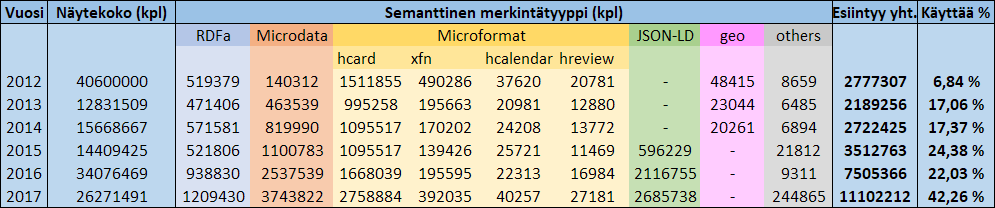
\includegraphics[width=15cm]{images/taulukko.png}
\caption{Bizerin tilastojen pohalta laadittu kooste \cite{rdfa_usage}. \label{images/taulukko}}
\end{figure}

\begin{figure}[htb]
\centering
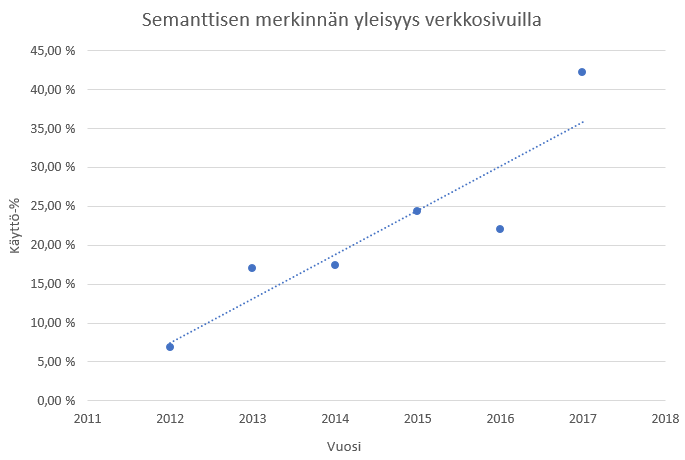
\includegraphics[width=13cm]{images/verkkosivut.png}
\caption{Edellisen taulukon pohjalta laadittu kuvaaja. \label{images/verkkosivut}}
\end{figure}
\clearpage

Kuvaajan trendikäyrä on johdettu yhteensä yli 140 miljoonan verkkosivustonäytteen pohjalta. Semanttisen tiedon yleistyminen on siis selvästi kasvava trendi. Bizerin tilastoja tukee vuonna 2010 tehty vastaavanlainen tiedonkeräys. Goel ja Gupta (2010) keräsivät miljoona näytettä, joista 42 605 sivua (eli 4,3 \%) käytti joko Microformat tai RDFa merkintää \cite{Google}. Tulos sijoittuu Bizerin tilastojen pohjalta johdetun lineaarisen trendikäyrän läheisyyteen.

Vuonna 2014 julkaistu HTML5-merkintäkieli sisältää semanttisia merkintöjä. Esimerkiksi elementit \textit{header}, \textit{main} ja \textit{footer} voitaisiin kaikki korvata rakenteensa puolesta \textit{div}-elementillä, mutta tällöin elementtien sisällöstä ei voida päätellä mitään. Uudet elementit, kuten \textit{article}, \textit{form} ja \textit{figure} vihjaavat tietokoneelle tiedon sisällöstä ja merkityksestä eli semantiikasta \cite{html5}. Näin esimerkiksi Googlen indeksoijat (engl. crawlers) kykenevät tunnistamaan verkkosivulla esiintyvän materiaalin tyypin \cite{html5}. HTML5:n tarjoamat ominaisuudet on otettu laajalti käyttöön, joten nykyisin semantiikkaa hyödyntävien verkkosivustojen määrän voidaan nähdä olevan edellisiä tilastoja suurempi. Semanttisia elementtejä on kuitenkin rajallinen määrä, joten HTML5:n avulla ei voida määritellä kaiken tiedon semantiikkaa.

\subsection{Semanttisen webin arkkitehtuuri}
Tietotekniikan yhteydessä arkkitehtuurilla viitataan ratkaisujen jäsentelyyn eli rakenteeseen. Semanttinen web koostuu selkeistä komponenteista, joten voidaan puhua, että semanttisella internetillä on arkkitehtuuri. Tim-Berners lee esitteli vuonna 2000 semanttisen webin arkkitehtuurin kuva \ref{images/sweb-stack.png} mukaisena. Pinomallissa ajatuksena oli jatkaa kehitystä aina edellisen tason päälle, jolloin tekniikoihin nähdyt investoinnit säilyisivät semanttisen webin kehittyessä. Ajatus kuitenkin vaatii, että tekniikat olisivat ikuisia ja aina yhteensopivia uusien kanssa, mikä ei ole käytännössä mahdollista \cite{stack}. Tästä syystä vuoden 2000 pinomalli ei ole realistinen ja sen tilalle on esitetty kuva \ref{images/sweb-stack.png} mallia.

% Side by side figures
\begin{figure}[htb]
\begin{minipage}[b]{0.48\linewidth}
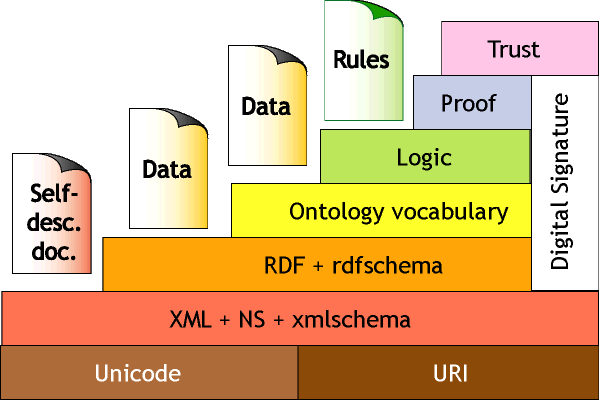
\includegraphics[width=\linewidth]{images/sweb-stack.png}
\caption{2000-luvun malli \cite{stack_bl} \label{images/sweb-stack.png}}
\end{minipage}
\hfill
\begin{minipage}[b]{0.48\linewidth}
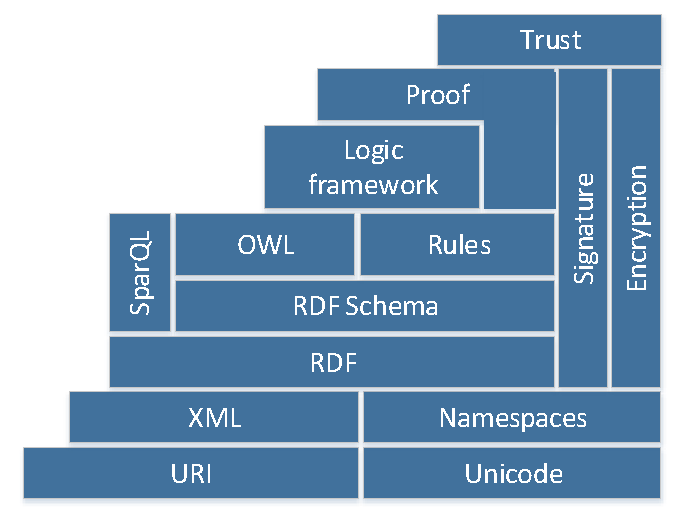
\includegraphics[width=\linewidth]{images/Semantic_web_stack_one_col.pdf}
\caption{2005-luvun malli \cite{stack} \label{images/Semantic_web_stack_one_col.pdf}}
\end{minipage}%
\end{figure}

Merkittävin ominaisuus uudessa pinomallissa on sen jakautuminen useampiin pinoihin. Tämä sallii tekniikoiden muuttua ja vaihtua vapaammin ilman oletusta, että ne säilyisivät ikuisesti \cite{stack}. Vaikka malli on esitetty vuonna 2005, niin se vastaa edelleen nykypäivän (vuoden 2018) arkkitehtuuria melko hyvin. W3C:n ylläpitämiä standardeja on päivitetty, joten tekniikat eivät ole päässeet vanhenemaan ja niitä hyödynnetään edelleen. Jälkimmäistä pinomallia voidaan siis edelleen käyttää lähtökohtana sovellusten rakenteen suunnittelussa.

%%==============================================================================
\section{Yhteenveto}

% Vastaa kysymyksiin.
% Katso arvostelumatriisi ja tee sen mukaan !!!

Semanttinen web on ihmisten ja tietokoneiden yhteisesti hyödynnettävissä oleva tietoresurssi. Tavallisessa internetissä materiaali on lähtökohtaisesti suunnattu ihmisille, jolloin tietokoneet eivät kykene ymmärtämään esittämäänsä materiaalia. Semanttinen web pyrkii muuntamaan internetissä esiintyvän materiaalin sellaiseen muotoon, jota myös tietokoneet kykenevät ymmärtämään. Tämän seurauksena tiedon hyödynnettävyys mahdollisuudet paranevat, koska voidaan rakentaa sovelluksia, jotka hyödyntävät tietokoneen ymmärtämää tietoa.

Tiedon muuntaminen tietokoneiden ymmärtämään eli semanttiseen muotoon tapahtuu W3C:n ylläpitämien standardien avulla. Keskeisiä tiedon esittämiseen ja määritykseen liittyviä standardeja ovat RDF, RDFS ja OWL. RDF-tietomuoto mahdollista joustavan tavan esittää ihmiseltä peräisin olevaa tietoa. Tiedonkohteisiin viitataan yksiselitteisten URI:en avulla. Usein tietoa halutaan kuitenkin ilmaista yleisellä tasolla, milloin suoria URI-viittauksia ei voida käyttää. Tällöin tiedon kuvailuun hyödynnetään RDF Schemaa, jonka avulla voidaan määritellä luokkia ja luokkien ominaisuuksia. RDFS määrittelee kaikista tarpeellisimmat semanttisen webin tiedonkuvausmekanismit, mutta RDFS:n määritykset eivät ole aina riittäviä. Tällöin tiedon kuvaamiseen voidaan hyödyntää ilmaisuvoimaisempaa OWL:ia. Kun tieto määritellään riittävän hyvin, niin tietokone kykenee tekemään itsenäisiä päätelmiä tiedon pohjalta. Vaadittu määrittelyn tarkkuus riippuu sovelluksesta, joten sovellus määrää tarpeelliset tekniikat. Kaikki tekniikat vastaavat tiettyihin ongelmiin, minkä vuoksi mikään tekniikka ei ole turha, mutta yksittäisessä sovelluksessa ei välttämättä tarvita kaikkia tekniikoita.

Tiedon esittämisen ja kuvailun lisäksi tietoa halutaan usein myös tallentaa. RDF-tietomuodossa olevaa tietoa voidaan tallentaa tehokkaasti graafimaisiin triplestore tietokantoihin. Triplestore tietokantojen tehokkuus johtuu RDF-tiedon linkittyneestä rakenteesta. Triplestore tietokannoista tietoa haetaan tehokkaasti RDF:lle suunnatun SPARQL-kyselykielen avulla. Standardin mukaisia graafimaisia tietokantoja on helpompi linkittää yhteen kuin perinteisiä relaatioitietokantoja. Tämä johtuu tietokantojen rakenteesta. Relaatiotietokannoissa rakenne voi vaihdella hyvinkin paljon sovellusten kesken, kun taas graafimaiset tietokannat ovat keskenään yhtenäisempiä. Siksi toisiinsa helposti linkitettäviä graafimaisia tietokantoja suositaan yhdistetyn tiedon yhteydessä.

Laajoja tietämysverkkoja voidaan hyödyntää esimerkiksi silloin, kun haetaan vastauksia ihmisten esittämiin kysymyksiin. Tietoa linkittämällä on myös mahdollista tarjota käyttäjälle merkityksellistä tietoa, vaikka hän ei suoraan pyytäisikään sitä. Tietokoneymmärrettävä tieto tarjoaa monia sovellusmahdollisuuksia.







\clearpage
%%==============================================================================
%% Lähdeluettelo - toisesta tiedostosta
\bibliographystyle{myieeetran} %acm
\bibliography{bibliography.bib}
\clearpage
%%==============================================================================
\thesisappendix

\begin{changemargin}{-1.5cm}{-1.5cm}
\section{Laaja esimerkki \label{LiiteA}}

Tässä liitteessä on yhtenäinen Turtle-syntaksilla kirjoitettu ontologia esimerkki. Esimerkissä kuvataan kuvitteellisen pöytätietokoneen rakennetta. Esimerkin tarkoituksena on auttaa hahmottamaan työssä esiteltyjen tekniikoiden yhteiskäyttöä ja ontologioiden rakennetta, sillä tekstissä esiintyvät esimerkit ovat hyvin pelkistettyjä. Myös tämä esimerkki on yksinkertaistettu, jotta se mahtuu järkevälle määrälle sivuja. Alla on esitelty esimerkin karkea rakenne graafimaisessa muodossa. Graafissa ei ole esitelty esimerkin kaikkia määritelmiä.

\begin{figure}[htb]
\centering
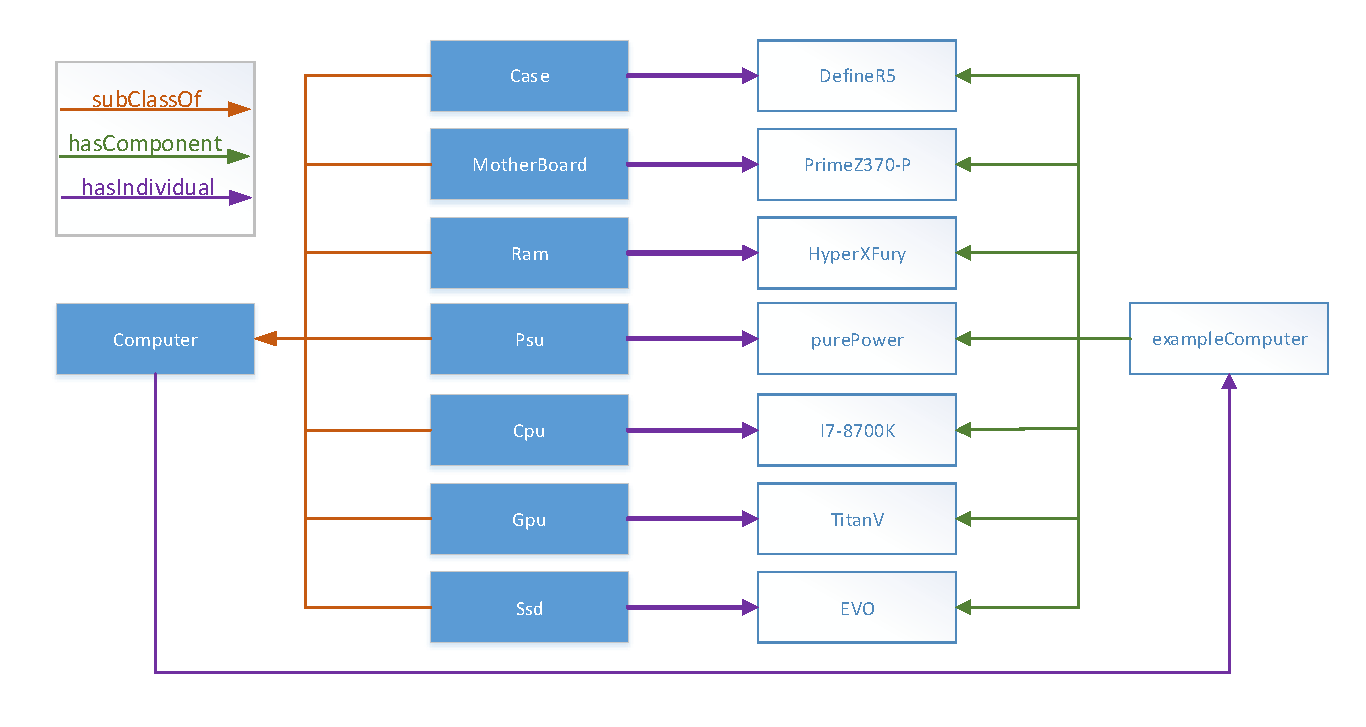
\includegraphics[width=15cm]{images/Computer_example.pdf}
\caption{Tietokone ontologian rakenne \label{images/taulukko}}
\end{figure}

\lstinputlisting[style=codeblock]{files/full_computer.owl}
\clearpage

\end{changemargin}
\end{document}
